%%%% Шаблон ВКР <<SPbPU-student-thesis-template>>  %%%%
%%
%%   Создан на основе глубокой переработки шаблона российских кандидатских и докторских диссертаций [1]. 
%%   
%%   Полный список различий может быть получен командами git.
%%   Лист авторов-составителей расположен в README.md файле.
%%   Подробные инструкции по использованию в [1,2].
%%   
%%   Рекомендуем установить TeX Live + TeXstudio
%%   <<Стандартная>> компиляция 2-3 РАЗА с помощью pdflatex + biber (для библиографии)     
%%  
%%%% Student thesis template <<SPbPU-student-thesis-template>> %%%%
%%
%%   Created on the basis of deepl modifification of the Russian candidate and doctorate thesis template [1]. 
%%   
%%   Full list of differences can be achieved by git commands.
%%   List of template authors can be seen in the README.md file.
%%   Detailed instructions of usage, see, please in [1,2].
%%     
%%   [1] github.com/AndreyAkinshin/Russian-Phd-LaTeX-Dissertation-Template 
%%   [2] Author_guide_SPBPU-student-thesis-template.pdf
%%   
%%   It is recommended to install TeX Live + TeXstudio   
%%   Default compilation 2-3 TIMES with pdflatex + biber (for the bibliography)
%%  
%%%% Preamble start %%%%  
%%
%%   Please, do not modify files in the preamble
%%
\newcommand*{\anyptfilebase}{template_settings/bpfont} 
\newcommand*{\anyptsize}{14} 		 
\RequirePackage[l2tabu,orthodox]{nag} 
\documentclass[extrafontsizes,a4paper,*pt,oneside,openany]{memoir}
\input{template_settings/common/setup}               
\input{template_settings/common/packages}  
\input{template_settings/Dissertation/dispackages}         
\input{template_settings/Dissertation/userpackages}         
\input{template_settings/Dissertation/setup}               
\input{template_settings/Dissertation/preamblenames}       
\input{template_settings/common/styles}    
\input{template_settings/Dissertation/disstyles}           
\input{template_settings/Dissertation/userstyles}          
\input{template_settings/biblio/bibliopreamble}
\input{template_settings/Dissertation/inclusioncontrol}
\input{template_settings/common/TO-DO-list}

%%
%%%% Preamble end %%%%  % лучше не редактировать / please, keep unmodified

\setcounter{docType}{1} % лучше не редактировать / please, keep unmodified

%%%% Настройки автора / Author settings
%% 
\input{my_folder/my_settings} % добавляем свои команды / update your commands


\usepackage{register}

\usepackage{url}

\begin{document} % начало документа


%%% Внесите свои данные - Input your data
%%
%%
\newcommand{\Author}{Д.В.\,Пешков} % И.О. Фамилия автора 
\newcommand{\AuthorFull}{Пешков Даниил Валерьевич} % Фамилия Имя Отчество автора
\newcommand{\AuthorFullDat}{Пешкову Даниилу Валерьевичу} % Фамилия Имя Отчество автора в дательном падеже (Кому? Студенту...)
\newcommand{\AuthorFullVin}{Пешкова Даниила Валерьевича} % в винительном падеже (Кого? что?  Програмиста ...)
\newcommand{\AuthorPhone}{+7-999-238-48-11} % номер телефорна автора для оперативной связи  
\newcommand{\Supervisor}{А.А.\,Лавров} % И. О. Фамилия научного руководителя
\newcommand{\SupervisorFull}{Фамилия Имя Отчество} % Фамилия Имя Отчество научного руководителя
\newcommand{\SupervisorVin}{И.О.\,Фамилию} % И. О. Фамилия научного руководителя  в винительном падеже (Кого? что? Руководителя ...)
\newcommand{\SupervisorJob}{должность} %
\newcommand{\SupervisorJobVin}{должность} % в винительном падеже (Кого? что?  Програмиста ...)
\newcommand{\SupervisorDegree}{степень} %
\newcommand{\SupervisorTitle}{звание} % 
%%
%%
%Руководитель, утверждающий задание
\newcommand{\Head}{И.О.\,Фамилия} % И. О. Фамилия руководителя подразделения (руководителя ОП)
\newcommand{\HeadDegree}{Должность руководителя}% Только должность:   
%Руководитель %ОП 
%Заведующий % кафедрой
%Директор % Высшей школы
%Зам. директора
\newcommand{\HeadDep}{M} % заменить на краткую аббревиатуру подразделения или оставить пустым, если утверждает руководитель ОП

%%% Руководитель, принимающий заявление
\newcommand{\HeadAp}{И.О.\,Фамилия} % И. О. Фамилия руководителя подразделения (руководителя ОП)
\newcommand{\HeadApDegree}{Должность руководителя}% Только должность:   
%Руководитель ОП 
%Заведующий кафедрой
%Директор Высшей школы
\newcommand{\HeadApDep}{O} % заменить на краткую аббревиатуру подразделения или оставить пустым, если утверждает руководитель ОП
%%% Консультант по нормоконтролю
\newcommand{\ConsultantNorm}{И.О.\,Фамилия} % И. О. Фамилия консультанта по нормоконтролю. ТОЛЬКО из числа ППС!
\newcommand{\ConsultantNormDegree}{должность, степень} %   
%%% Первый консультант
\newcommand{\ConsultantExtraFull}{Фамилия Имя Отчетство} % Фамилия Имя Отчетство дополнительного консультанта 
\newcommand{\ConsultantExtra}{И.О.\,Фамилия} % И. О. Фамилия дополнительного консультанта 
\newcommand{\ConsultantExtraDegree}{должность, степень} % 
\newcommand{\ConsultantExtraVin}{И.О.\,Фамилию} % И. О. Фамилия дополнительного консультанта в винительном падеже (Кого? что? Руководителя ...)
\newcommand{\ConsultantExtraDegreeVin}{должность, степень} %  в винительном падеже (Кого? что? Руководителя ...)
%%% Второй консультант
\newcommand{\ConsultantExtraTwoFull}{Фамилия Имя Отчетство} % Фамилия Имя Отчетство дополнительного консультанта 
\newcommand{\ConsultantExtraTwo}{И.О.\,Фамилия} % И. О. Фамилия дополнительного консультанта 
\newcommand{\ConsultantExtraTwoDegree}{должность, степень} % 
\newcommand{\ConsultantExtraTwoVin}{И.О.\,Фамилию} % И. О. Фамилия дополнительного консультанта в винительном падеже (Кого? что? Руководителя ...)
\newcommand{\ConsultantExtraTwoDegreeVin}{должность, степень} %  в винительном падеже (Кого? что? Руководителя ...)
\newcommand{\Reviewer}{И.О.\,Фамилия} % И. О. Фамилия резензента. Обязателен только для магистров.
\newcommand{\ReviewerDegree}{должность, степень} % 
%%
%%
\renewcommand{\thesisTitle}{Тема выпускной квалификационной работы}
\newcommand{\thesisDegree}{работа бакалавра}% дипломный проект, дипломная работа, магистерская диссертация %c 2020
\newcommand{\thesisTitleEn}{Title of the thesis} %2020
\newcommand{\thesisDeadline}{дд.мм.202X}
\newcommand{\thesisStartDate}{дд.мм.202X}
\newcommand{\thesisYear}{202X}
%%
%%
\newcommand{\group}{N} % заменить вместо N номер группы
\newcommand{\thesisSpecialtyCode}{ХХ.ХХ.ХХ}% код направления подготовки
\newcommand{\thesisSpecialtyTitle}{Наименование направления подготовки} % наименование направления/специальности
\newcommand{\thesisOPPostfix}{YY} % последние цифры кода образовательной программы (после <<_>>)
\newcommand{\thesisOPTitle}{Наименование направленности (профиля) образовательной программы}% наименование образовательной программы
%%
%%
\newcommand{\institute}{
Название института
%Институт компьютерных наук и~технологий
%Гуманитарный институт
%Инженерно-строительный институт
%Институт биомедицинских систем и технологий
%Институт металлургии, машиностроения и транспорта
%Институт передовых производственных технологий
%Институт прикладной математики и механики
%Институт физики, нанотехнологий и телекоммуникаций
%Институт физической культуры, спорта и туризма
%Институт энергетики и транспортных систем
%Институт промышленного менеджмента, экономики и торговли
}%
%%
%%




%%% Задание ключевых слов и аннотации
%%
%%
%% Ключевых слов от 3 до 5 слов или словосочетаний в именительном падеже именительном падеже множественного числа (или в единственном числе, если нет другой формы) по правилам русского языка!!!
%%
%%
\newcommand{\keywordsRu}{Стилевое оформление сайта, управление контентом, php, MySQL, архитектура системы} % ВВЕДИТЕ ключевые слова по-русски
%%
%%
\newcommand{\keywordsEn}{Style registration, content management, php, MySQL, system architecture} % ВВЕДИТЕ ключевые слова по-английски
%%
%%
%% Реферат ОТ 1000 ДО 1500 знаков на русский или английский текст
%%
%Реферат должен содержать:
%- предмет, тему, цель ВКР;
%- метод или методологию проведения ВКР:
%- результаты ВКР:
%- область применения результатов ВКР;
%- выводы.

\newcommand{\abstractRu}{В данной работе изложена сущность подхода к созданию динамического информационного портала на основе использования открытых технологий Apache, MySQL и PHP. Даны общие понятия и классификация IT-систем такого класса. Проведен анализ систем-прототипов. Изучена технология создания указанного класса информационных систем. Разработана конкретная программная реализация динамического информационного портала на примере портала выбранной тематики...} % ВВЕДИТЕ текст аннотации по-русски
%%
%%
\newcommand{\abstractEn}{In the given work the essence of the approach to creation of a dynamic information portal on the basis of use of open technologies Apache, MySQL and PHP is stated. The general concepts and classification of IT-systems of such class are given. The analysis of systems-prototypes is lead. The technology of creation of the specified class of information systems is investigated. Concrete program realization of a dynamic information portal on an example of a portal of the chosen subjects is developed...} % ВВЕДИТЕ текст аннотации по-английски


%%% РАЗДЕЛ ДЛЯ ОФОРМЛЕНИЯ ПРАКТИКИ
%Место прохождения практики
\newcommand{\PracticeType}{Отчет о прохождении % 
	%стационарной производственной (технологической (проектно-технологической)) %
	такой-то % тип и вид ЗАМЕНИТЬ
	практики}

\newcommand{\Workplace}{СПбПУ, ИКНТ, ВШИСиСТ} % TODO Rename this variable

% Даты начала/окончания
\newcommand{\PracticeStartDate}{%
дд.мм.гггг%
%	22.06.2020
}%
\newcommand{\PracticeEndDate}{%
	дд.мм.гггг%
%	18.07.2020%
}%
%%

\newcommand{\School}{
	Название высшей школы
%	Высшая школа интеллектуальных систем и~суперкомпьютерных~технологий 
}
\newcommand{\practiceTitle}{Тема практики}


%% ВНИМАНИЕ! Необходимо либо заменить текст аннотации (ключевых слов) на русском и английском, либо удалить там весь текст, иначе в свойства pdf-отчета по практике пойдет шаблонный текст.

%%% Не меняем дальнейшую часть - Do not modify the rest part
%%
%%
%%
%%
\ifnumequal{\value{docType}}{1}{% Если ВКР, то...
	\newcommand{\DocType}{Выпускная квалификационная работа}
	\newcommand{\pdfDocType}{\DocType~(\thesisDegree)} %задаём метаданные pdf файла
	\newcommand{\pdfTitle}{\thesisTitle}
}{% Иначе 
	\newcommand{\DocType}{\PracticeType}
	\newcommand{\pdfDocType}{\DocType} %задаём метаданные pdf файла
	\newcommand{\pdfTitle}{\practiceTitle}
}%
\newcommand{\HeadTitle}{\HeadDegree~\HeadDep}
\newcommand{\HeadApTitle}{\HeadApDegree~\HeadApDep}
\newcommand{\thesisOPCode}{\thesisSpecialtyCode\_\thesisOPPostfix}% код образовательной программы
\newcommand{\thesisSpecialtyCodeAndTitle}{\thesisSpecialtyCode~\thesisSpecialtyTitle}% Код и наименование направления/специальности
\newcommand{\thesisOPCodeAndTitle}{\thesisOPCode~\thesisOPTitle} % код и наименование образовательной программы
%%
%%
\hypersetup{%часть болка hypesetup в style
		pdftitle={\pdfTitle},    % Заголовок pdf-файла
		pdfauthor={\AuthorFull},    % Автор
		pdfsubject={\pdfDocType. Шифр и наименование направления подготовки: \thesisSpecialtyCodeAndTitle. \abstractRu},      % Тема
		pdfcreator={LaTeX, SPbPU-student-thesis-template},     % Приложение-создатель
%		pdfproducer={},  % Производитель, Производитель PDF % будет выставлена автоматически
		pdfkeywords={\keywordsRu}
}
%%
%%
%% вспомогательные команды
\newcommand{\firef}[1]{рис.\ref{#1}} %figure reference
\newcommand{\taref}[1]{табл.\ref{#1}}	%table reference
%%
%%
%% Архивный вариант задания ключевых слов, аннотации и благодарностей 
% Too hard to export data from the environment to pdf-info
% https://tex.stackexchange.com/questions/184503/collecting-contents-of-environment-and-store-them-for-later-retrieval
%заменить NewEnviron на newenvironment для распознавания команды в TexStudio
%\NewEnviron{keywordsRu}{\noindent\MakeUppercase{\BODY}}
%\NewEnviron{keywordsEn}{\noindent\MakeUppercase{\BODY}}
%\newenvironment{abstractRu}{}{}
%\newenvironment{abstractEn}{}{}
%\newenvironment{acknowledgementsRu}{\par{\normalfont \acknowledgements.}}{}
%\newenvironment{acknowledgementsEn}{\par{\normalfont \acknowledgementsENG.}}{}


%%% Переопределение именований %%% Не меняем - Do not modify
%\newcommand{\Ministry}{Минобрнауки России} 
\newcommand{\Ministry}{Министерство науки и высшего образования Российской~Федерации} %с 2020
\newcommand{\SPbPU}{Санкт-Петербургский политехнический университет Петра~Великого}
\newcommand{\SPbPUOfficialPrefix}{Федеральное государственное автономное образовательное учреждение высшего образования}
\newcommand{\SPbPUOfficialShort}{ФГАОУ~ВО~<<СПбПУ>>}
%% Пробел между И. О. не допускается.
\renewcommand{\alsoname}{см. также}
\renewcommand{\seename}{см.}
\renewcommand{\headtoname}{вх.}
\renewcommand{\ccname}{исх.}
\renewcommand{\enclname}{вкл.}
\renewcommand{\pagename}{Pages}
\renewcommand{\partname}{Часть}
\renewcommand{\abstractname}{\textbf{Аннотация}}
\newcommand{\abstractnameENG}{\textbf{Annotation}}
\newcommand{\keywords}{\textbf{Ключевые слова}}
\newcommand{\keywordsENG}{\textbf{Keywords}}
\newcommand{\acknowledgements}{\textbf{Благодарности}}
\newcommand{\acknowledgementsENG}{\textbf{Acknowledgements}}
\renewcommand{\contentsname}{Content} % 
%\renewcommand{\contentsname}{Содержание} % (ГОСТ Р 7.0.11-2011, 4)
%\renewcommand{\contentsname}{Оглавление} % (ГОСТ Р 7.0.11-2011, 4)
\renewcommand{\figurename}{Рис.} % Стиль СПбПУ
%\renewcommand{\figurename}{Рисунок} % (ГОСТ Р 7.0.11-2011, 5.3.9)
\renewcommand{\tablename}{Таблица} % (ГОСТ Р 7.0.11-2011, 5.3.10)
%\renewcommand{\indexname}{Предметный указатель}
\renewcommand{\listfigurename}{Список рисунков}
\renewcommand{\listtablename}{Список таблиц}
\renewcommand{\refname}{\fullbibtitle}
\renewcommand{\bibname}{\fullbibtitle}

\newcommand{\chapterEnTitle}{Сhapter title} % <- input the English title here (only once!) 
\newcommand{\chapterRuTitle}{Название главы}          % <- введите 
\newcommand{\sectionEnTitle}{Section title} %<- input subparagraph title in english
\newcommand{\sectionRuTitle}{Название подраздела} % <- введите название подраздела по-русски
\newcommand{\subsectionEnTitle}{Subsection title} % - input subsection title in english
\newcommand{\subsectionRuTitle}{Название параграфа} % <- введите название параграфа по-русски
\newcommand{\subsubsectionEnTitle}{Subsubsection title} % <- input subparagraph title in english
\newcommand{\subsubsectionRuTitle}{Название подпараграфа} % <- введите название подпараграфа по-русски % Заполнить сведения, 
										 % в т.ч. ключевые слова и аннотацию.

%%% Титульник ВКР / Thesis title 
%%
%% добавить лист в pdf-навигацию 
%% add to pdf navigation menu
%%
\pdfbookmark[-1]{\pdfTitle}{tit}
%%
\thispagestyle{empty}%
\makeatletter
\newgeometry{top=2cm,bottom=2cm,left=3cm,right=1cm,headsep=0cm,footskip=0cm}
\savegeometry{NoFoot}%
\makeatother


%%% Распечатать версию документа / Print document version
%%
%\begin{flushright}
%	\vspace{0pt plus0.1fill}
%	\boxed{\small
%		\begin{tabular}{r} 
%			\textbf{Пример ВКР <<SPbPU-student-thesis-template>>.} %\\ % перенос на новую строку
%			\textbf{Версия от \today % \; время:  \currenttime. % время версии
%			}
%		\end{tabular}
%	} %end boxed
%	\vspace*{-5pt} % раскомментировать, если не хватает места
%	\vspace{0pt plus0.1fill} % раскоментировать, если хватает места
%\end{flushright}

{\centering%
	\Ministry\\
	\SPbPU\\
	{%\bfseries %2020 - указание на изменения, которые могут быть введены в 2020 году
		\institute}
\par}%


\vspace{0pt plus1fill} %число перед fill = кратность относительно некоторого расстояния fill, кусками которого заполнены пустые места


\noindent
\begin{minipage}{\linewidth}
	\vspace{\mfloatsep} % интервал 
	\begin{tabularx}{\linewidth}{Xl}
	&Работа допущена к защите     \\
	&\HeadTitle     \\			
	&\underline{\hspace*{0.1\textheight}} \Head     \\
	&<<\underline{\hspace*{0.05\textheight}}>> \underline{\hspace*{0.1\textheight}} \thesisYear~г.  \\ 
	\end{tabularx}
	\vspace{\mfloatsep} % интервал 	
\end{minipage}


\vspace{0pt plus2fill} %


{\centering%
	
	\MakeUppercase{\bfseries{}\DocType} \\ 
	\MakeUppercase{\thesisDegree}%


\intervalS% %ОБЯЗАТЕЛЬНО ДОБАВИТЬ ОТСТУП, ЕСЛИ ХВАТАЕТ МЕСТА
{\centering%
	\MakeUppercase{\bfseries{\thesisTitle}}}%

}\par%
%\noindent
{\centering%
\intervalS% %ОБЯЗАТЕЛЬНО ДОБАВИТЬ ОТСТУП, ЕСЛИ ХВАТАЕТ МЕСТА
%по специальности % для специалистов
	по направлению  \thesisSpecialtyCodeAndTitle{}\\% для бакалавров и магистров 
%\noindent Направленность  % для специалистов
по образовательной программе\\


\thesisOPCodeAndTitle % для бакалавров и магистров
% Лучше по~профилю, но что делать, так составили Положение
\par%
}\par%




\vspace{4mm plus2fill}%

\noindent
\begin{tabularx}{\linewidth}{lXl}
	Выполнил              &	   &             \\
	студент гр.~\group     & \emph{<подпись>}   & \Author     \\[\mfloatsep]

	Руководитель 		  &    &             \\
	\SupervisorJob,		  &    &             \\
	\SupervisorDegree, \SupervisorTitle 	  &  \emph{<подпись>}  & \Supervisor \\[\mfloatsep]
	
	Консультант	  &    & 			 \\
	\ConsultantExtraDegree 	  &  \emph{<подпись>}  & \ConsultantExtra\\[\mfloatsep]
	
	Консультант  &    &  \\   	
	по нормоконтролю  		 	  & \emph{<подпись>}   & \ConsultantNorm  % обязателен
\end{tabularx} %


%
\vspace{0pt plus4fill}% 


\begin{center}%
Санкт-Петербург\\
\thesisYear
\end{center}%
\restoregeometry
\newpage					 % Титульный лист
										 % Убираем footnotes, консультанта, если нет

%%%% Начало оформления заголовка - оставить без изменений !!! %%%%
\input{my_folder/task_settings}	% настройки - начало 
	
				{%\normalfont %2020
						\MakeUppercase{\SPbPU}}\\
				\institute

\par}\intervalS% завершает input

				\noindent
				\begin{minipage}{\linewidth}
				\vspace{\mfloatsep} % интервал 	
				\begin{tabularx}{\linewidth}{Xl}
					&УТВЕРЖДАЮ      \\
					&\HeadTitle     \\			
					&\underline{\hspace*{0.1\textheight}} \Head     \\
					&<<\underline{\hspace*{0.05\textheight}}>> \underline{\hspace*{0.1\textheight}} \thesisYear г.  \\  
				\end{tabularx}
				\vspace{\mfloatsep} % интервал 	
				\end{minipage}

\intervalS{\centering\bfseries%

				ЗАДАНИЕ\\
				на выполнение %с 2020 года 
				%по выполнению % до 2020 года
				выпускной квалификационной работы


\intervalS\normalfont%

				студенту \uline{\AuthorFullDat{} гр.~\group}


\par}\intervalS%
%%%%
%%%% Конец оформления заголовка  %%%%
 	
	
	
\begin{enumerate}[1.]
	\item Тема работы: {\expandafter \ulined \thesisTitle.}
	%\item Тема работы (на английском языке): \uline{\thesisTitleEn.} % вероятно после 2021 года
	\item Срок сдачи студентом законченной работы: \uline{\thesisDeadline.} 
	\item Исходные данные по работе: \uline{Техническая документация на систему суб-наносекундной синхронизации <<White Rabbit Project>>.}%
	%\printbibliographyTask % печать списка источников % КОММЕНТИРУЕМ ЕСЛИ НЕ ИСПОЛЬЗУЕТСЯ
	% В СЛУЧАЕ, ЕСЛИ НЕ ИСПОЛЬЗУЕТСЯ МОЖНО ТАКЖЕ ЗАЙТИ В setup.tex и закомментировать \vspace{-0.28\curtextsize}
	\item Содержание работы (перечень подлежащих разработке вопросов):
	\begin{enumerate}[label=\theenumi\arabic*.]
		\item Изучить техническую документацию по процедуре калибровки узлов сети White Rabbit.
		\item Изучить техническую документацию на используемые в калибраторе электронные узлы.
		\item Портировать используемые открытые модули под целевую ПЛИС.
		\item Реализовать модули для проведения измерений при помощи стробирования.
		\item Спроектировать систему на кристалле и интегрировать в неё используемые аппаратные модули.
		\item Написать драйвера для используемой периферии.
		\item Протестировать и отладить полученное управляющее устройство на опытном образце калибратора, при
				необходимости осуществить доработку.
		
	\end{enumerate}
	\item Перечень графического материала (с указанием обязательных чертежей):\\
	 Отсутствует.
	
		\item Консультанты по работе:
		\begin{enumerate}[label=\theenumi\arabic*.] 
		\item  \uline{\emakefirstuc{\ConsultantExtraDegree}, \ConsultantExtra.} % закомментировать при необходимости, идёт первый по порядку.
		\item \uline{\emakefirstuc{\ConsultantNormDegree} \ConsultantNorm{} (нормоконтроль).} %	Обязателен для всех студентов
	\end{enumerate}
		\item Дата выдачи задания: \uline{\thesisStartDate.}
\end{enumerate}

\intervalS%можно удалить пробел

Руководитель ВКР \uline{\hspace*{0.1\textheight} \Supervisor}


\intervalS%можно удалить пробел

Консультант  \uline{\hspace*{0.1\textheight}\ConsultantExtra}


\intervalS%можно удалить пробел

%Консультант по нормоконтролю \uline{\hspace*{0.1\textheight} \ConsultantNorm}%ПОКА НЕ ТРЕБУЕТСЯ, Т.К. ОН У ВСЕХ ПО УМОЛЧАНИЮ

Задание принял к исполнению \uline{\thesisStartDate}

\intervalS%можно удалить пробел

Студент \uline{\hspace*{0.1\textheight}  \Author}



\input{my_folder/task_settings_restore}	% настройки - конец					 % Задание 
										 % Для сдачи в высшую школу компилируем двухсторонний My_task.tex 
										 % После подписания задания изменение его содержания и оформления запрещено

%% Не менять - Do not modify
%%\input{my_folder/summary_settings} 
\chapter*[Count-me]{Реферат} % * - не нумеруем
\thispagestyle{empty}% удаляем параметры страницы
%\setcounter{sumPageFirst}{\value{page}}
%sumPageFirst \arabic{sumPageFirst}
%
%
%% Возможность проверить другие значения счетчиков - debugging
%\ref*{TotPages}~с.,
%\formbytotal{mytotalfigures}{рисун}{ок}{ка}{ков},
%\formbytotal{mytotaltables}{таблиц}{у}{ы}{},
%There are \TotalValue{mytotalfigures} figures in this document
%There are \TotalValue{mytotalfiguresInApp} figuresINAPP in this document
%There are \TotalValue{mytotaltables} tables in this document
%There are \TotalValue{mytotaltablesInApp} figuresINAPP in this document
%There are \TotalValue{myappendices} appendix chapters in this document
%\total{citenum}~библ. наименований.



%% Для того, чтобы значения счетчиков корректно отобразились, необходимо скомпилировать файл 2-3 раза
На \total{mypages}~c.,  
\formbytotal{myfigures}{рисун}{ок}{ка}{ков},
\formbytotal{mytables}{таблиц}{у}{ы}{},
\formbytotal{myappendices}{приложен}{ие}{ия}{ий}%.  

%\noindent
{\MakeUppercase{Ключевые слова: \keywordsRu}.} % Ключевые слова из renames.tex

Тема выпускной квалификационной работы: <<\thesisTitle>>.


\abstractRu % Аннотация из renames.tex



\printTheAbstract % не удалять


\total{mypages}~pages, 
\total{myfigures}~figures, 
\total{mytables}~tables,
\total{myappendices}~appendices%.

%\noindent
{\MakeUppercase{Keywords: \keywordsEn}.} % Ключевые слова из renames.tex 
	
The subject of the graduate qualification work is <<\thesisTitleEn>>.
	
	
\abstractEn % Аннотация из renames.tex



%% Не менять - Do not modify
\thispagestyle{empty}
%\setcounter{sumPageLast}{\value{page}} %сохранили номер последней страницы Задания
%\setcounter{sumPages}{\value{sumPageLast}-\value{sumPageFirst}}
%sumPageLast \arabic{sumPageLast}
%
%sumPages \arabic{sumPages}
%\restoregeometry % восстанавливаем настройки страницы
%\input{my_folder/summary_settings_restore}	% настройки - конец			 	 % Реферат 
										 % Убираем footnotes, дубли команд \abstractEn и \abstractRu 
										

\input{my_folder/contents}  	         % Оглавление


\chapter*{Введение} % * не проставляет номер
\addcontentsline{toc}{chapter}{Введение} % вносим в содержание

Для надёжного функционирования распределённых систем потоковой обработки данных, работающих в
режиме реального времени, на исполняемые в них операции накладываются строгие временные ограничения.
Многочисленные узлы таких систем могут находиться друг от друга на значительных расстояниях, 
что приводит к длительным (и не всегда одинаковым) задержкам при передаче сигналов между ними.
Возникающие задержки приводят к рассинхронизации работы устройств систем, что влечёт за собой 
возникновение потенциально некорректных результатов выполнения операций. 

С целью согласования всех устройств и обеспечения общего представления времени во всей сети применяются 
системы синхронизации часов. Такие системы гарантируют, что часы всех устройств сети отсчитывают время с 
одинаковой скоростью (выдают одинаковые показания в каждый момент времени).

Для передачи информации при синхронизации могут использоваться различные протоколы.
Наибольшее распространение получили следующие два: NTP (Network Time Protocol) и PTP (Precision Time Protocol).
Протокол NTP способен обеспечивать точность синхронизации времени до одной миллисекунды, а протокол PTP – до десяти миллисекунд. 

Протоколы NTP и PTP не подходят для случая, когда необходима синхронизация с субнаносекундной точностью. Например, 
такая высокая точность требуется в распределённых системах, применяемых в экспериментах физики высоких энергий.
Там они используются для потоковой обработки информации, поступающей с детекторов и ускорителей частиц. 

Системы субнаносекундной синхронизации применяются в Большом Адронном Коллайдере, расположенным в ЦЕРН, в Швейцарии. Они также
планируются к применению в строящемся комплексе «NICA» Объединённого института ядерных исследований (ОИЯИ) в Дубне. 
Другим приложением субнаносекундной синхронизации являются системы радиочастотного позиционирования,
использующие технологию сверхширокополосной связи (UWB) и алгоритм позиционирования TDoA (Time Difference of Arrival).

Основные положения работы описаны в [1].

\textbf{Цель работы:} разработка управляющего устройства для устройства, выполняющего калибровку систем субнаносекундной синхронизации.

\textbf{Решаемые в данной работе задачи:} портирование и интеграция существующих открытых модулей в систему на кристалле, 
реализация модулей для проведения измерений по принципу стробоскопического осциллографа, написание драйверов для используемой периферии,
написания управляющей программы для процессорного ядра, тестирование и отладка.

Разработка аппаратной части проекта выполнена на языке System Verilog, управляющей программы -- на языке C. 
Для компиляции используется компилятор gcc под архитектуру RV32IM.	    	 % Введение

%% Начало основной части
\chapter{Анализ предметной области} \label{ch1}

\section{White Rabbit} \label{ch1:sec1}

White Rabbit -- система синхронизации часов. Разработана при сотрудничестве множества
институтов и компаний. Изначально проект был начат для улучшения текущей системы синхронизации в Церне.
Предполагалось использование для физических экспериментов, однако в процессе было создано обобщенное решение,
которое нашло своё применение в различных сферах.\\

\noindent Характеристики:

\begin{itemize}
	\item Суб-наносекундная точность
	\item Большое количество синхронизируемых узлов
	\item Расстояния в десятки километров
	\item Канал передачи между двумя узлами –- 1 Gbps
	\item Открытый исходный код\\
\end{itemize}

Достоинствами White Rabbit являются полностью открытый исходный код и аппаратура, а также 
использование существующих стандартов (Ethernet, PTP и т. д.).

\section{Калибровка}

Синхронизация в сети White Rabbit выполняется по протоколу WR PTP –- модифицированному протоколу PTP. (IEEE 1588).
Однако для достижения суб-наносекундной точности необходима дополнительная калибровка.

Обмен данными между двумя устройствами происходит по одной линии оптоволокна, работающей в полнодуплексном режиме.
Для передачи в одну и другую сторону используется свет с разной длиной волны, поэтому возникает асимметричность в
задержках распространения сигнала. Из-за этого устройство не может само определить задержки, отправив эхо запрос
другому устройству –- время распространения сигнала в одну и другую сторону не равны.

Определение коэффициента асимметричности оптоволокна позволит протоколу White Rabbit PTP обеспечить требуемую точность синхронизации устройств сети.

\begin{figure}[ht!] 
	\center
	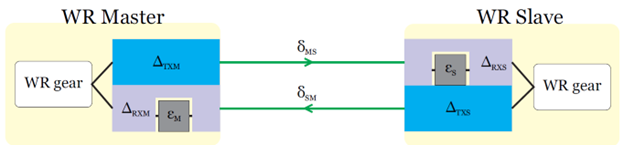
\includegraphics  {my_folder/images//conn_model}
	\caption{Модель соединения между двумя устройствами} 
	\label{fig:conn-model}  
\end{figure}

На \firef{fig:conn-model} изображены возникающие задержки, требующие калибровки. Внутри каждого устройства 
возникают задержки на приёме и отправке ($\Delta_{TXM},\Delta_{RXM},\Delta_{TXS},\Delta_{RXS}, \varepsilon_{M},\varepsilon_{S}$),
которые являются результатом задержек в SFP (Small Form-factor Pluggable) 
модуле, в электрических цепях и электронных компонентах. Эти задержки калибруются отдельно на каждом устройстве и не являются
предметом рассмотрения в данной работе.

Суммарная задержка распространения сигнала от ведущего устройства к ведомому устройству и обратно считается по формуле:

\begin{equation}
delay_{MM} = \Delta_{TXM} + \Delta_{RXS} + \varepsilon_{S} + \Delta_{TXS} + \Delta_{RXM} + \varepsilon_{M} + \delta_{MS} + \delta_{SM}
\end{equation}

В данной работе рассматривается калибровка задержек $\delta_{MS}$ и $\delta_{SM}$ – задержек распространения сигнала по оптоволокну.

Когда оптоволокно ещё не установлено, измерить задержки и вычислить коэффициент асимметричности можно без особых усилий.
Коэффициент асимметричности определяется, как:

\begin{equation}
	\alpha = \frac{\delta_{MS} - \delta_{SM}}{\delta_{SM}}
\end{equation}

Измеряется коэффициент при помощи дополнительного короткого оптоволокна, с известной задержкой (\firef{fig:meas-scheme-1}).

\begin{figure}[ht!] 
	\center
	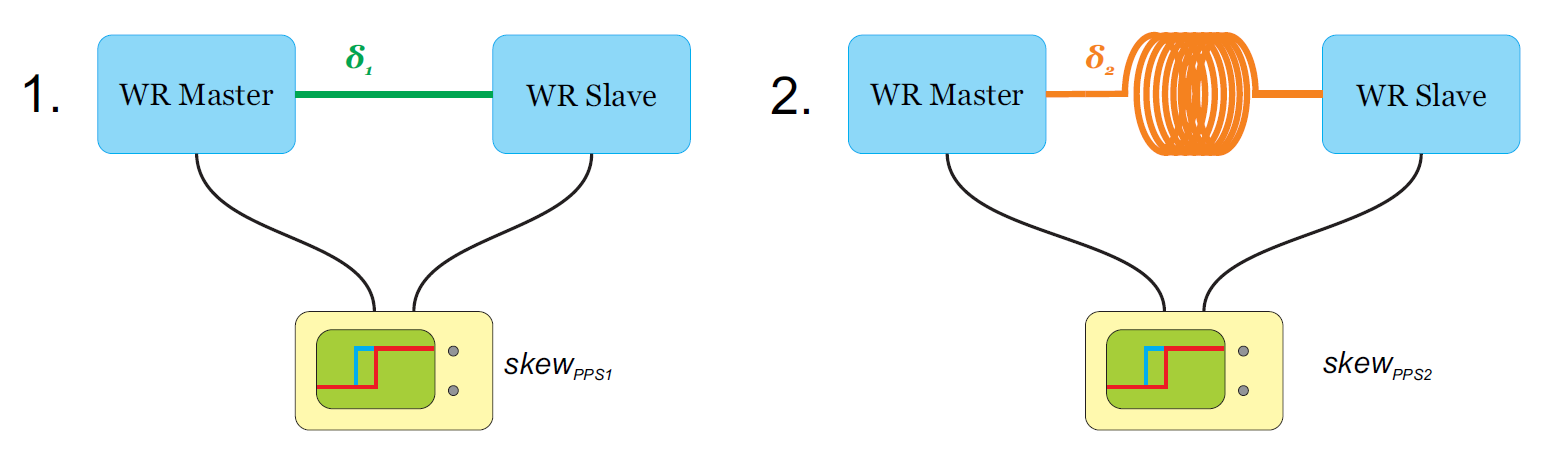
\includegraphics [scale=0.4] {my_folder/images//meas_scheme_1}
	\caption{Измерение асимметричности про помощи дополнительного оптоволокна} 
	\label{fig:meas-scheme-1}  
\end{figure}

Два устройства подключаются калибруемым оптоволокном ($\delta_{2}$) и дополнительным ($\delta_{1}$) отдельно, 
далее два устройства синхронизируются. После этого измеряется разность фаз синхросигналов 1-PPS
(Pulse Per Second), генерируемых ведущим и ведомым устройством. 

\begin{equation}
	skew_{PPS} = t_{PPS_S} - t_{PPS_M}\\
\end{equation}

По измеренным значениям можно определить коэффициент асимметричности, как:

\begin{equation}
	\label{eq:alpha}
	\alpha = \frac{2 \left( skew_{PPS2} - skew_{PPS1} \right) }{\frac{1}{2} \delta_2 - \left( skew_{PPS2} - skew_{PPS1} \right)}
\end{equation}


Однако существуют так же уже установленные линии, нуждающиеся в калибровке. В таких случаях описанный выше метод не подходит.

\begin{figure}[ht!] 
	\center
	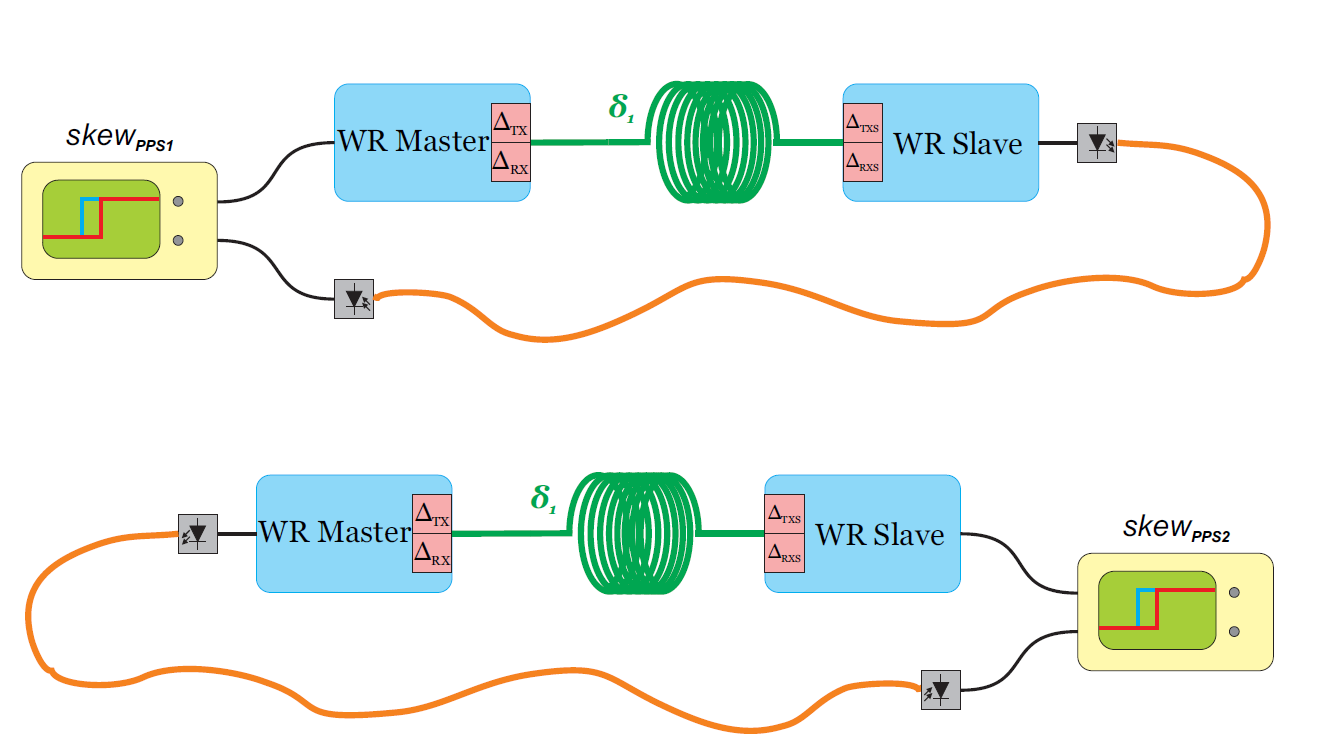
\includegraphics [scale=0.4] {my_folder/images//meas_scheme_2}
	\caption{Измерение асимметричности про помощи дополнительного оптоволокна} 
	\label{fig:meas-scheme-2}  
\end{figure}

В таких случаях применяется немного изменённый метод с подключением петли от выхода 1-PPS одного устройства к другому (\firef{fig:meas-scheme-2}). 
После синхронизации так же измеряются расхождения фронтов синхросигналов и усредняются.

\begin{equation}
	skew_{PPS} = \frac{1}{2} \left(skew_{PPS1} + skew_{PPS2} \right)
\end{equation}

Далее это значение может быть использовано для вычисления коэффициента по формуле \labelcref{eq:alpha}.

Разрабатываемое устройство служит для автоматизированного измерения разности фаз и выполнения калибровки.

\section{Актуальность}

Для процесса калибровки предполагается использовать устройство, способное измерять отрезки времени меньше, чем 1 нс, чтобы обеспечить
суб-наносекундную точность, т.е. иметь частоту дискретизации 1 GSa. Если применить правило <<пятикратного превышения частоты дискретизации>>, то
используемый осциллограф должен иметь частоту дискретизации выше 5 GSa. 

Цена осциллографов с такими характеристиками крайне высока. Актуальность данной работы заключается в том, что предлагается разработать
относительно бюджетное устройство, работающее по принципу стробоскопического осциллографа.
 
Сигналы PPS от калибруемых устройств являются периодическими. Это позволяет применить для их обнаружения, захвата и анализа устройство,
работающее по принципу стробоскопического осциллографа.

\section{Стробоскопический осциллограф}

Стробоскопические осциллографы предназначены для обнаружения, захвата и анализа периодических сигналов.
Принцип работы стробоскопического осциллографа проиллюстрирован на \firef{fig:stb-osc}.

\begin{figure}[ht!] 
	\center
	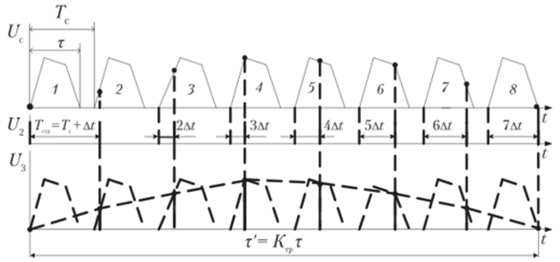
\includegraphics {my_folder/images//stb_osc}
	\caption{Измерение асимметричности про помощи дополнительного оптоволокна} 
	\label{fig:stb-osc}  
\end{figure}

Условные обозначения:

\begin{itemize}[label={}]
	\item $ U_{c} $ -- исследуемый периодический сигнал
	\item $ T_{c} $ -- период исследуемого сигнала
	\item $ \tau $ -- длительность исмпульса исследуемого сигнала
	\item $ \Delta t $ -- шаг считывания исследуемого сигнала
	\item $ U_{2} $ -- стробы осциллографа
	\item $ U_{3} $ -- снятая осциллограмма сигнала\\
\end{itemize}

Таким образом, для снятия очередной точки изменяется смещение $ \Delta t $.
Частота дискретизации определяется минимальным смещением, которое может задать осциллограф.
\FloatBarrier
\newpage	         	 % Глава 1
\ContinueChapterBegin % размещать главы <<подряд>> 
\chapter{Аппаратная платформа и алгоритм проведения измерений}
	
Управляющее устройство реализовано на базе ПЛИС, так как есть необходимость разрабатывать 
специфические аппаратные модули.\\

В качестве аппаратной платформы УУ (управляющее устройство) выступает ПЛИС серии
LittleBee китайского производителя Gowin Semiconductor -- GW1N-UV9QN88C6/I5.\\

\noindent Данная ПЛИС имеет следующие характеристики:\\


\begin{itemize}
	\item количество логических блоков LUT4 -- 8640 шт.
	\item количество триггеров -- 6480 шт.
	\item объём FLASH -- 408 Кбит
	\item количество блоков BSRAM -- 26 шт.
	\item объём блоков SRAM -- 468 Кбит
	\item количество блоков PLL (ФАПЧ) -- 2 шт.
	\item напряжение питания ядра -- 1.8–3.3 В
	\item количество доступных для пользователя выходов I/O -- 77
	\item среди них дифференциальных пар -- 19\\
\end{itemize}

\begin{figure}[ht!] 
	\center
	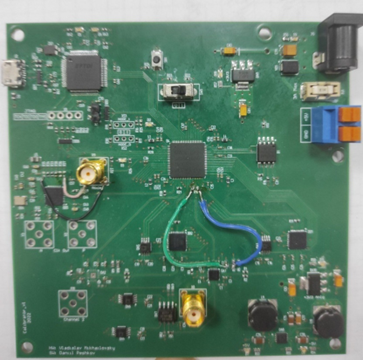
\includegraphics {my_folder/images//pcb}
	\caption{Печатная плата устройства} 
	\label{fig:pcb}  
\end{figure}

\begin{figure}[ht!] 
	\center
	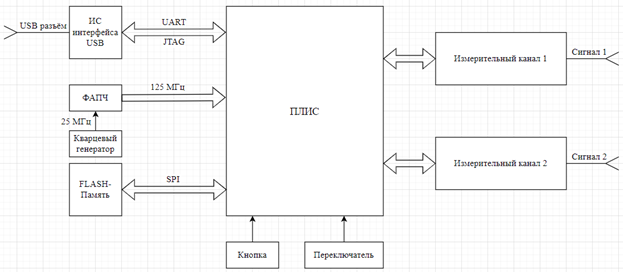
\includegraphics {my_folder/images//scheme_struct}
	\caption{Структурная схема устройства} 
	\label{fig:scheme-struct}  
\end{figure}

На \firef{fig:scheme-struct} изображена структурная схема устройства.
К УУ подключаются два измерительных канала, которыми необходимо управлять для проведения измерений.
ПЛИС тактируется высокостабильным тактовым сигналом с частотой 125 МГц. Связь с устройством верхнего уровня
осуществляется через FTDI чип FT2232H[5].

Перед разработкой УУ необходимо определить ОУ (объект управления), которым предстоит управлять.

\section{Измерительный канал}

\begin{figure}[ht!] 
	\center
	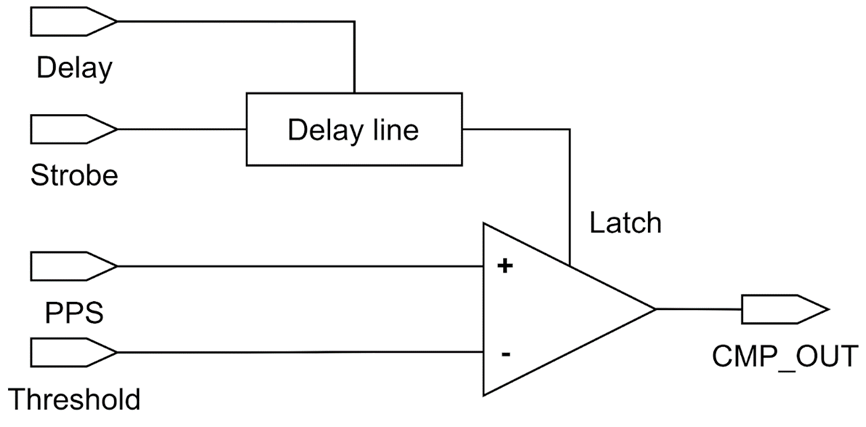
\includegraphics {my_folder/images//ch_func}
	\caption{Функциональная схема измерительного канала} 
	\label{fig:ch-func}  
\end{figure}

На \firef{fig:ch-func} приведена функциональная схема одного из измерительных каналов.


\begin{itemize}[label={}]
	\item Threshold -- пороговое напряжение сравнения на компараторе
	\item Delay -- настройка задержки сигнала на линии задержки (Delay line)
	\item Strobe -- стробы, выдаваемые УУ и защёлкивающее текущий результат сравнения компаратора.
	\item PPS -- измеряемый сигнал 1-PPS (В общем случае, может быть любой частоты, кратной либо 125 МГц,
		либо частоте внешнего тактового сигнала, подаваемого с SMA разъёма)\\
\end{itemize}

\section{Алгоритм проведения измерений}

Перед началом проведения измерения необходимо определить частоты измеряемого сигнала и найти его фронт.

\begin{figure}[ht!] 
	\center
	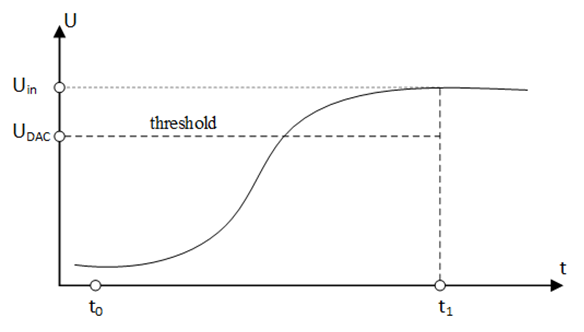
\includegraphics {my_folder/images//meas_alg}
	\caption{Измерение сигнала} 
	\label{fig:meas-alg}  
\end{figure}

Далее необходимо начать генерировать стробы с частотой измеряемого сигнала. Стробы блокируют
текущий выход компаратора, и на его выходе остаётся результат сравнения в момент прихода строба.
При помощи изменения задержки можно сдвигать измеряемую точку по оси OX.
Для поиска значения напряжения в измеряемой точке необходимо изменять пороговое напряжение сравнения
на компараторе.

На \firef{fig:meas-alg} приведён пример измерения. 
$ t_{0} $ -- точка от которой измеряется сигнал (момент прихода строба),
$ t_{1} $ -- измеряемая точка (момент прихода задержанного строба на компаратор).
Временной отрезок $ [t_{0}, t_{1}] $ задаётся линией задержки.
Если в момент защёлкивания на выходе компаратора логическая единица, значит измеряемое напряжение выше,
чем пороговое. Перед приходом следующего строба пороговое напряжение повышается.
Так продолжается до тех пор, пока на выходе компаратора не будет логического нуля.
В таком случае мы считаем, что измеряемая точка имеет значения напряжение равное пороговому.
Задержка увеличивается, и измеряется следующая точка. Таким образом снимается осциллограмма входного сигнала.


\section{Пороговое напряжение сравнения}

Для задания порогового напряжения используется DAC (Digital to analog converter) AD5662 от Analog Devices.
AD5662 -- 16-битный DAC с гарантированной точностью 12 бит[3].

%\begin{figure}[ht!] 
%	\center
%	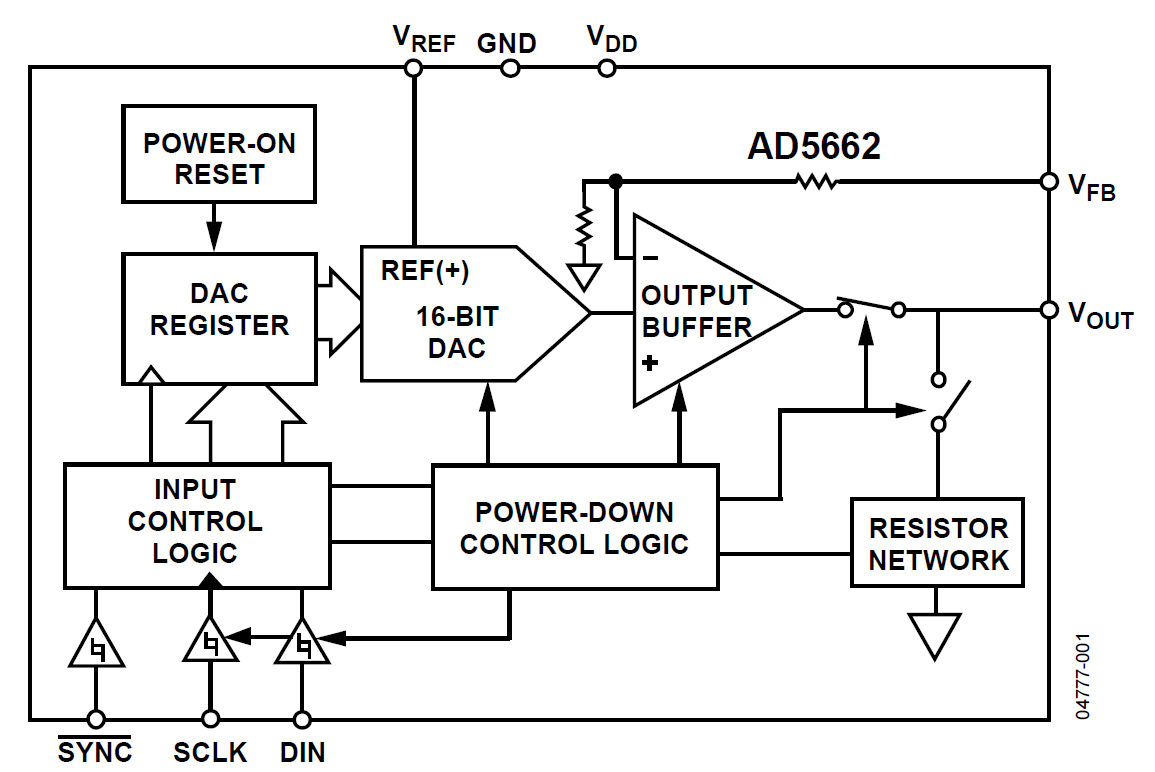
\includegraphics [scale=0.5] {my_folder/images//dac_func}
%	\caption{Функциональная схема AD5662} 
%	\label{fig:dac-func}  
%\end{figure}

С опорным напряжением 3.3 В, шаг изменения напряжения -- $ \frac{3.3}{2^{16}} \approx 50 $ мкВ.
Для задания напряжения используется интерфейс SPI (\firef{fig:dac-interface}).

\begin{figure}[ht!] 
	\center
	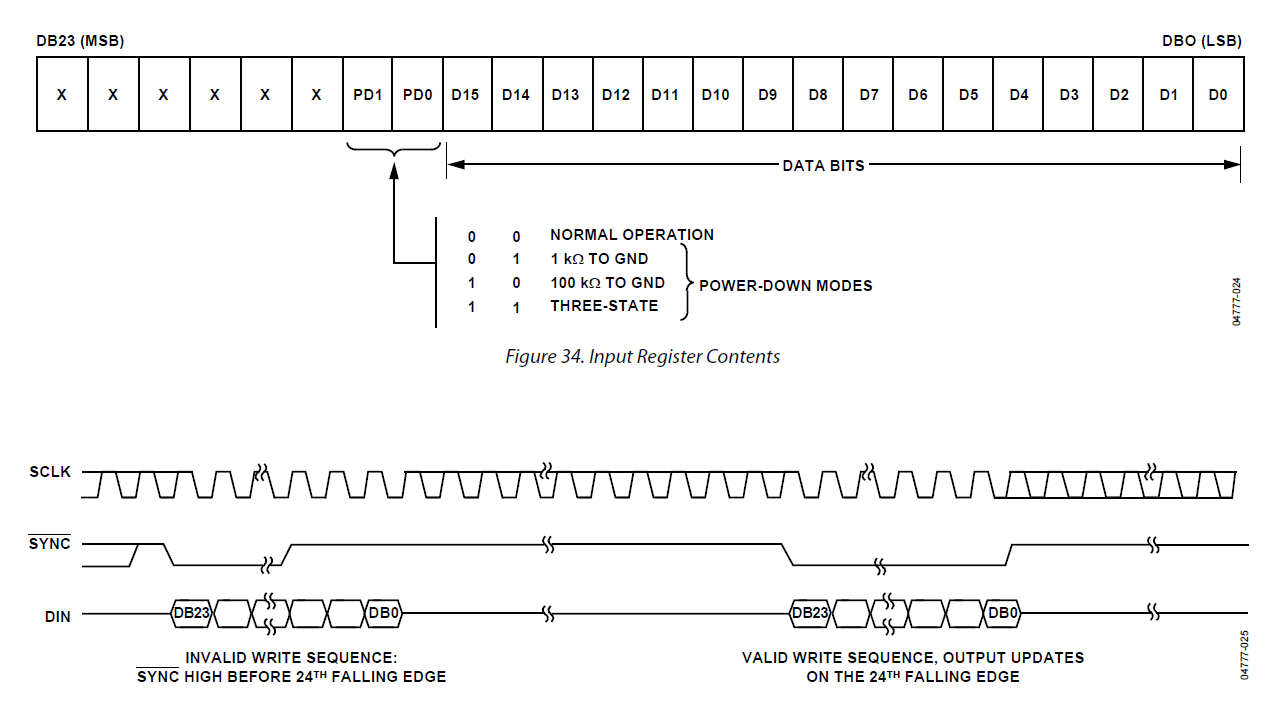
\includegraphics [scale=0.5] {my_folder/images//dac_interface}
	\caption{Интерфейс взаимодействия с AD5662} 
	\label{fig:dac-interface}  
\end{figure}

При напряжении питания 3.3 В максимальная частота сигнала SCLK -- 20 МГц. Максимальное время установки
выходного напряжения -- 10 мкс (обычно 8 мкс).

\section{Линия задержки}

Для сдвига задержки строба используется микросхема SY100EP196V от Microchip[12]. Задержка задаётся 10-битным
цифровым кодом с шагом $ \approx $ 10 пс (\firef{fig:dline-code}). Так же есть аналоговый вход FTUNE, которым можно точнее точнее подстраивать
задержку (\firef{fig:dline-ftune}) (на данный момент не используется).

\begin{figure}[ht!] 
	\center
	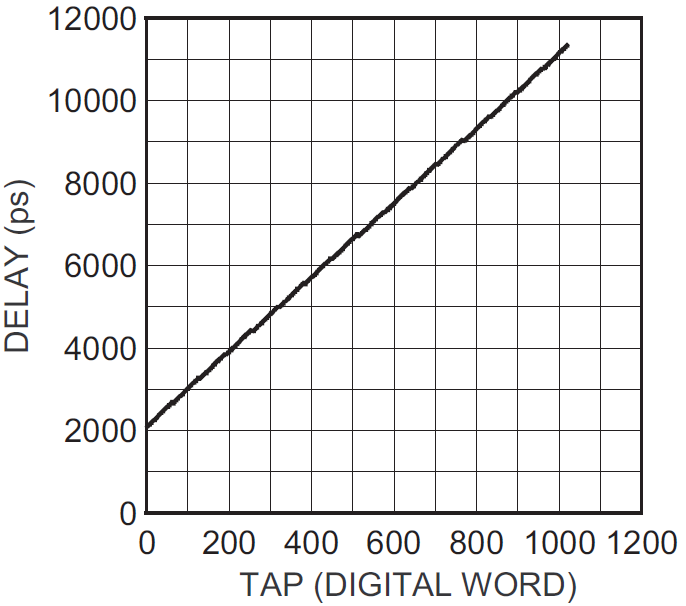
\includegraphics [scale=0.6] {my_folder/images//dline_code}
	\caption{Задержка, задаваемая цифровым входом} 
	\label{fig:dline-code}  
\end{figure}

\begin{figure}[ht!] 
	\center
	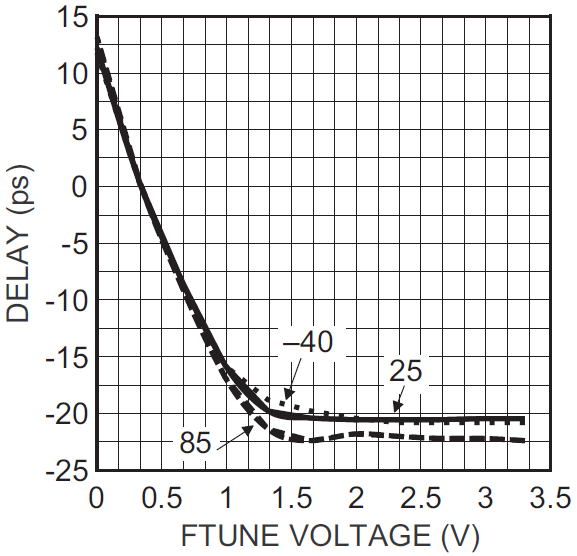
\includegraphics [scale=0.6] {my_folder/images//dline_ftune}
	\caption{Подстройка задержки через аналоговый вход FTUNE} 
	\label{fig:dline-ftune}  
\end{figure}


\section{Компаратор}

Для сравнения используется компаратор ADCMP582 от Analog Devices[2]. Основным параметром, который необходимо учесть является $ t_{PL} $ (\firef{fig:cmp-wave}).

\begin{figure}[ht!] 
	\center
	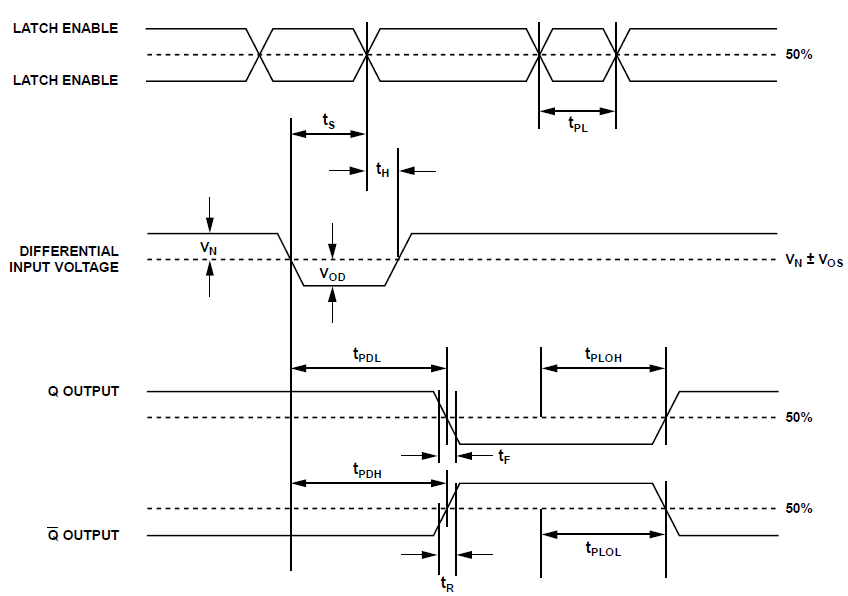
\includegraphics [scale=0.7] {my_folder/images//cmp_wave}
	\caption{Временная диаграмма ADCMP582} 
	\label{fig:cmp-wave}  
\end{figure}
\FloatBarrier

$ t_{PL} $ -- минимальное время, в течение которого вход защёлки (Latch Enable) должен быть высоким, чтобы результат сравнения попал на выход компаратора.

\newpage	         	 % Глава 2
\chapter{Разработка аппаратного описания управляющего устройства}

Все исходные коды аппаратных описаний находятся в директории \emph{/rtl/}.

\section{Описание верхнего уровня}

Описание верхнего уровня находится в файле \emph{/rtl/calsoc\_top.sv}.\\

Управляющее устройство реализовано в виде СнК (Система на кристалле) (\firef{fig:calsoc}) на базе открытого процессорного
ядра \emph{PicoRV32}, основанного на открытой архитектуре RISC-V.

Все периферийные модули подключаются к ядру через шину \emph{Wishbone}. Арбитраж на шине выполняет открытый модуль
\emph{wbxbar}.

\begin{figure}[ht!] 
	\center
	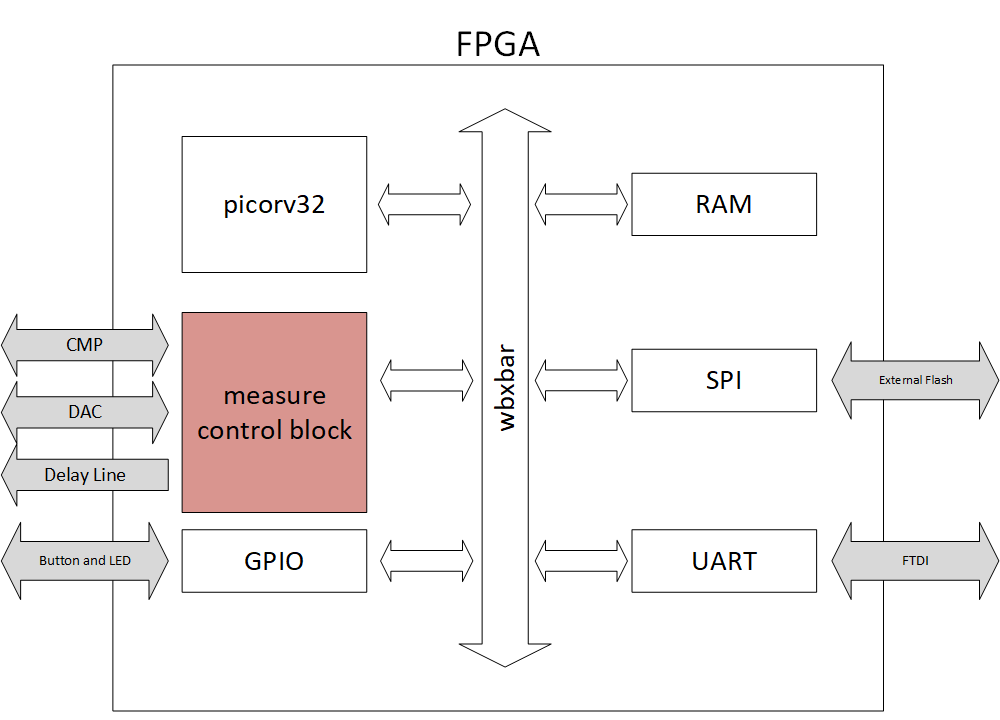
\includegraphics [scale=0.7] {my_folder/images//calsoc}
	\caption{Структурная схема СнК} 
	\label{fig:calsoc}  
\end{figure}

Все периферийные устройства разделяют между собой общее адресное пространство.

\begin{itemize}[label={}]
	\item 0x00000000 -- 0x00FFFFFF -- RAM 
	\item 0x01000000 -- 0x01FFFFFF -- ROM загрузичка
	\item 0x02000000 -- 0x02FFFFFF -- GPIO
	\item 0x03000000 -- 0x03FFFFFF -- UART1
	\item 0x04000000 -- 0x04FFFFFF -- память программы
	\item 0x05000000 -- 0x05FFFFFF -- измерительный модуль
\end{itemize}


\section{Измерительный модуль}

Измерительный модуль выдаёт все необходимые управляющие сигналы для проведения измерений и логически разделён на несколько компонентов (\firef{fig:mu-struct}):

\begin{itemize}
	\item \emph{stb\_gen} -- модуль, измеряющий частоту сигнала и генерирующий стробы
	\item \emph{ch\_measure\_ctl} -- модуль, непосредственно управляющий измерением одного канала
	\item \emph{spi\_master} -- модуль, реализующий взаимодействие с AD5662
	\item \emph{sc\_fifo} -- FIFO, накапливающее измеренные значения
\end{itemize}

\begin{figure}[ht!] 
	\center
	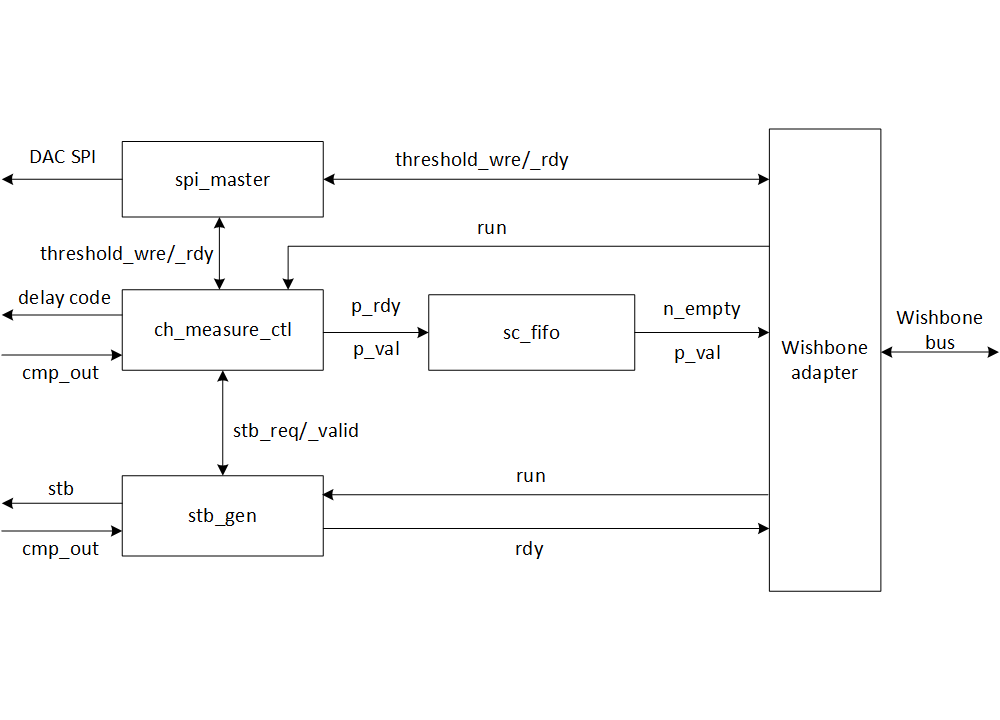
\includegraphics [scale=0.7] {my_folder/images//mu_struct}
	\caption{Структурная схема измерительного модуля (для одного канала)} 
	\label{fig:mu-struct}  
\end{figure}

Все описанные ранее модули подключены в модуле верхнего уровня \emph{measure\_unit}. В нём же
реализована вся логика управлением проведением измерений через шину Wishbone.

Далее будет отдельно рассмотрен каждый модуль.

\subsection{Модуль stb\_gen}

Для определения частоты измеряемого сигнала необходимо измерить время между двумя фронтами.
Для измерения используется 32-разрядный счётчик, один отсчёт которого равняется 8 нс (125 МГц).

Реализация <<в лоб>> не может работать стабильно на целевой ПЛИС из-за задержек на цепочке переносов в 
32-разрядном сумматоре. Для корректной работы на такой частоте необходимо конвейеризировать счётчик (\firef{fig:t-cnt}).

\begin{figure}[ht!] 
	\center
	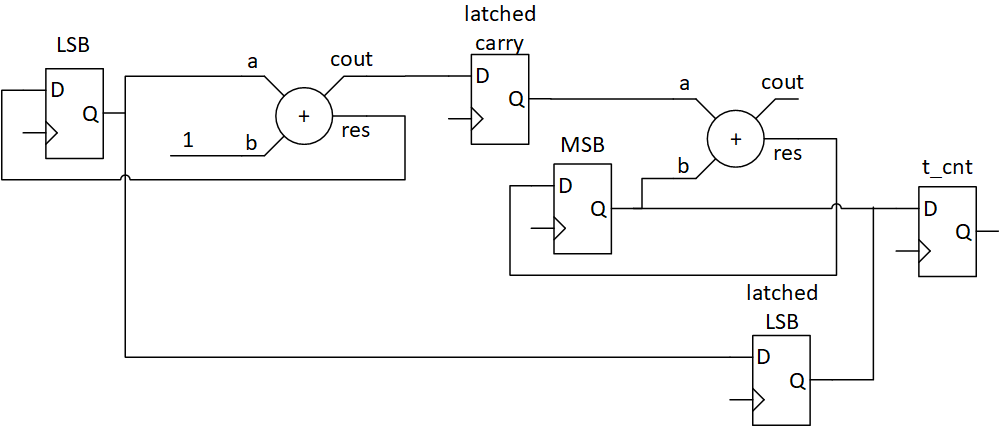
\includegraphics [scale=0.7] {my_folder/images//t_cnt}
	\caption{Конвейерный 32-х разрядный счётчик} 
	\label{fig:t-cnt}  
\end{figure}

К младшим байтам (регистр \emph{LSB}) каждый такт прибавляется 1, текущее значение младших байт защёлкивается в регистре \emph{latched LSB}.
При переполнении, перенос защёлкивается в регистре \emph{latched carry}. К старшим байтам (регистр \emph{MSB}) прибавляется сохранённый перенос из-за
младших байт. Выход счётчика -- комбинация значений регистров \emph{MSB} и \emph{latched LSB}.

\begin{flushright}
Листинг 3.1. Реализация на языке System Verilog
\end{flushright}
\lstset{
	numbersep = 5pt,
	stepnumber = 1
}
\begin{lstlisting}
// pipelined counter

	logic [T_CNT_WIDTH/2-1 : 0] high_bytes = 0;
	logic [T_CNT_WIDTH/2-1 : 0] latched_low_bytes = 0;
	logic [T_CNT_WIDTH/2-1 : 0] low_bytes = 0;
	logic [T_CNT_WIDTH/2-1 : 0] low_bytes_plus_1;
	logic carry;

	assign {carry, low_bytes_plus_1} = low_bytes + 1;

	//incrementing low bytes
	always_ff @(posedge clk_i, negedge arst_i) 
		if (~arst_i) low_bytes = 0;
		else low_bytes <= low_bytes_plus_1;

	//latching low bytes for 1 cycle
	always_ff @(posedge clk_i, negedge arst_i) 
		if (~arst_i) latched_low_bytes = 0;
		else latched_low_bytes <= low_bytes;

	logic latched_carry = 0;

	//latching carry
	always_ff @(posedge clk_i, negedge arst_i) 
		if (~arst_i) latched_carry = 0;
		else latched_carry <= carry;

	//adding latched carry to high bytes
	always_ff @(posedge clk_i, negedge arst_i)
		if (~arst_i) high_bytes = 0;
		else high_bytes <= high_bytes + latched_carry;

	//seting t_cnt
	always_ff @(posedge clk_i, negedge arst_i) 
		if (~arst_i) t_cnt = 0;
		else t_cnt <= {high_bytes, latched_low_bytes};
\end{lstlisting}

\begin{figure}[ht!] 
	\center
	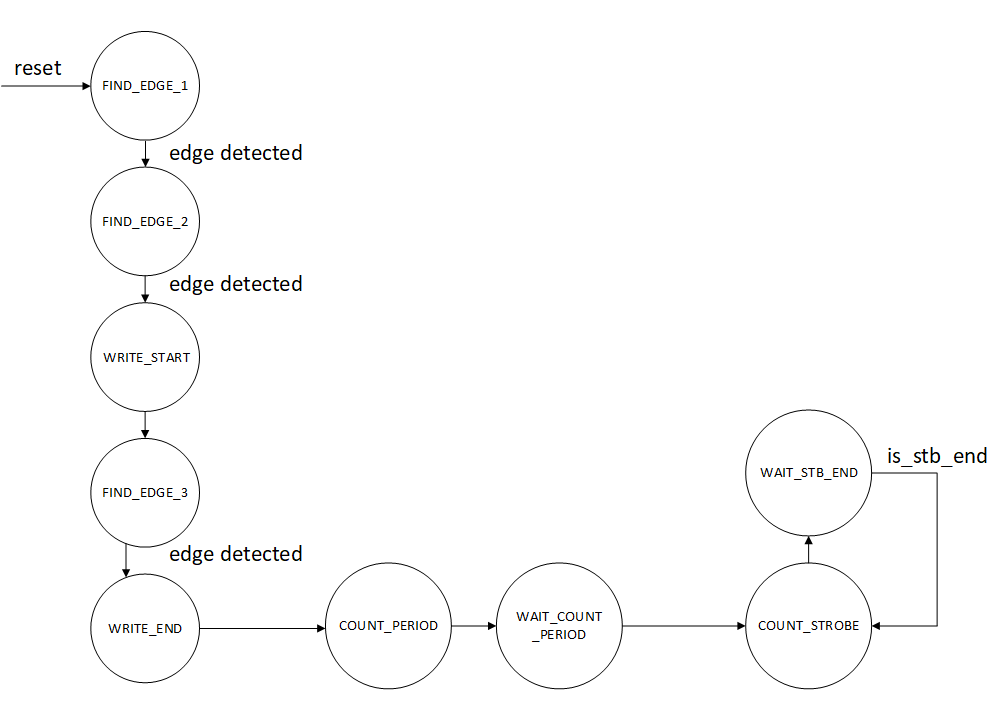
\includegraphics [scale=0.7] {my_folder/images//stb_gen_fsm}
	\caption{Конечный автомат модуля \emph{stb\_gen}} 
	\label{fig:stb-gen-fsm}  
\end{figure}

\FloatBarrier

Нас \firef{fig:stb-gen-fsm} представлен конечный автомат модуля \emph{stb\_gen}. Вся логика максимально упрощена, так как, если
на одной регистровой передаче будет много комбинаторной логики, при синтезе под целевую ПЛИС не получится выдержать требуемые $ t_{setup} $ и $ t_{hold} $.

\begin{itemize}[label={}]
	\item FIND\_EDGE\_1 -- состояние после сброса, ожидание первого фронта на входе \emph{sig\_i} 
	\item FIND\_EDGE\_2 -- ожидание второго фронта на входе \emph{sig\_i} 
	\item WRITE\_START -- запись текущего значения \emph{t\_cnt} в \emph{t\_start}
	\item FIND\_EDGE\_3 -- ожидание третьего фронта на входе \emph{sig\_i}
	\item WRITE\_END -- запись текущего значения \emph{t\_cnt} в \emph{t\_end}
	\item COUNT\_PERIOD -- вычисление периода сигнала ($ \emph{t\_end} - \emph{t\_start}) $
	\item WAIT\_COUNT\_PERIOD -- задержка на 1 такт
	\item COUNT\_STROBE -- начало расчёта времени начала и конца отрицательного импульса на выходе стробы
	\item WAIT\_STB\_END -- ожидание конца стробы и переход к расчёту новой\\
\end{itemize}

Таким образом, модуль определяет частоту входного сигнала и начинает бесконечно выдавать стробы.

Помимо 32-х разрядного счётчика, конвейеризация была необходима для всех операций с 32-х битными числами. В модуле \emph{two\_cycle\_32\_adder}
реализован двухтактный сумматор, однако использованный подход идентичен тому, что используется в счётчике.

Отдельного упоминания стоит оптимизация операции проверки на равенство двух чисел. Для этого необходимо сравнить попарно все биты
чисел, что выполняется параллельно и не должно увеличивать максимальный путь, однако при синтезе получалась цепочка с последовательным
сравнением всех разрядов (\firef{fig:eq}).\\

\begin{figure}[ht!] 
	\center
	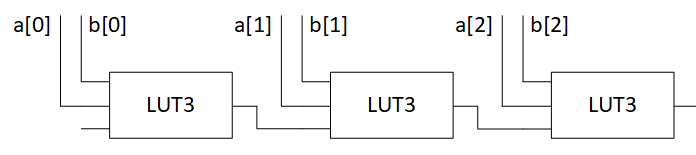
\includegraphics [scale=0.7] {my_folder/images//eq}
	\caption{Реализация сравнения при синтезе} 
	\label{fig:eq}  
\end{figure}

\FloatBarrier

Для исправления этого пришлось явно заменить операцию сравнения на исключающее ИЛИ и свёртку по ИЛИ-НЕ.

\begin{flushright}
Листинг 3.2. Реализация сравнения
\end{flushright}
\lstset{
	numbersep = 5pt,
	stepnumber = 1
}
\begin{lstlisting}
always_ff @(posedge clk_i) is_zero_hold_start_lo <=  ~|(t_cnt[15:0] ^ latched_zero_hold_res[15:0]);  //t_cnt == latched_zero_hold_res;
	always_ff @(posedge clk_i) is_zero_hold_start_hi <=  ~|(t_cnt[31:16] ^ latched_zero_hold_res[31:16]);  //t_cnt == latched_zero_hold_res;
	always_ff @(posedge clk_i) is_zero_hold_start <= is_zero_hold_start_lo & is_zero_hold_start_hi; 
\end{lstlisting}

При работе модуль не выдаёт стробы, а держит компаратор в защёлкнутом состоянии. Для запроса стробы используется пара сигналов
\emph{stb\_req\_i} и \emph{stb\_valid\_o}. При выдаче стробы, с компаратора снимается защёлка на короткое время, после чего устанавливается обратно.

Для тестирования модуля были написаны тестбенчи \emph{tb\_stb\_gen.sv} и \emph{tb2\_stb\_gen.sv}. На \firef{fig:tb-stb-gen} и \firef{fig:tb-stb-gen-out}
представлены результаты моделирования.

\begin{figure}[ht!] 
	\center
	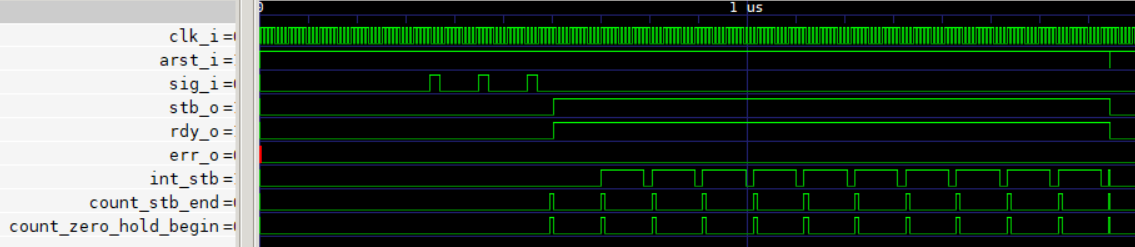
\includegraphics  [scale=0.7] {my_folder/images//tb_stb_gen}
	\caption{Пример определения частоты входного сигнала} 
	\label{fig:tb-stb-gen}  
\end{figure}

\begin{figure}[ht!] 
	\center
	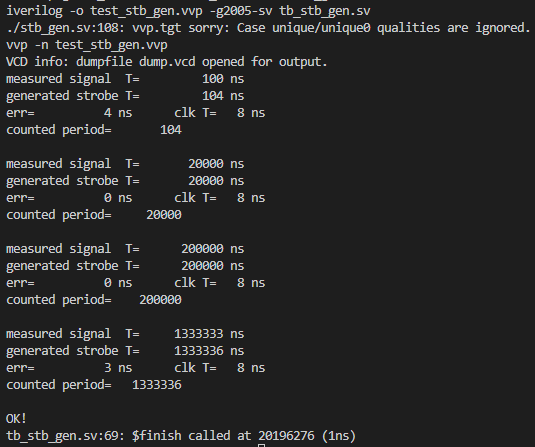
\includegraphics  [scale=0.8] {my_folder/images//tb_stb_gen_out}
	\caption{Вывод в консоль при симуляции} 
	\label{fig:tb-stb-gen-out}  
\end{figure}
\FloatBarrier

Видно, что сигналы с периодом, кратным 8 нс измеряются корректно, при измерении других -- ошибка меньше 8 нс.

\begin{figure}[ht!] 
	\center
	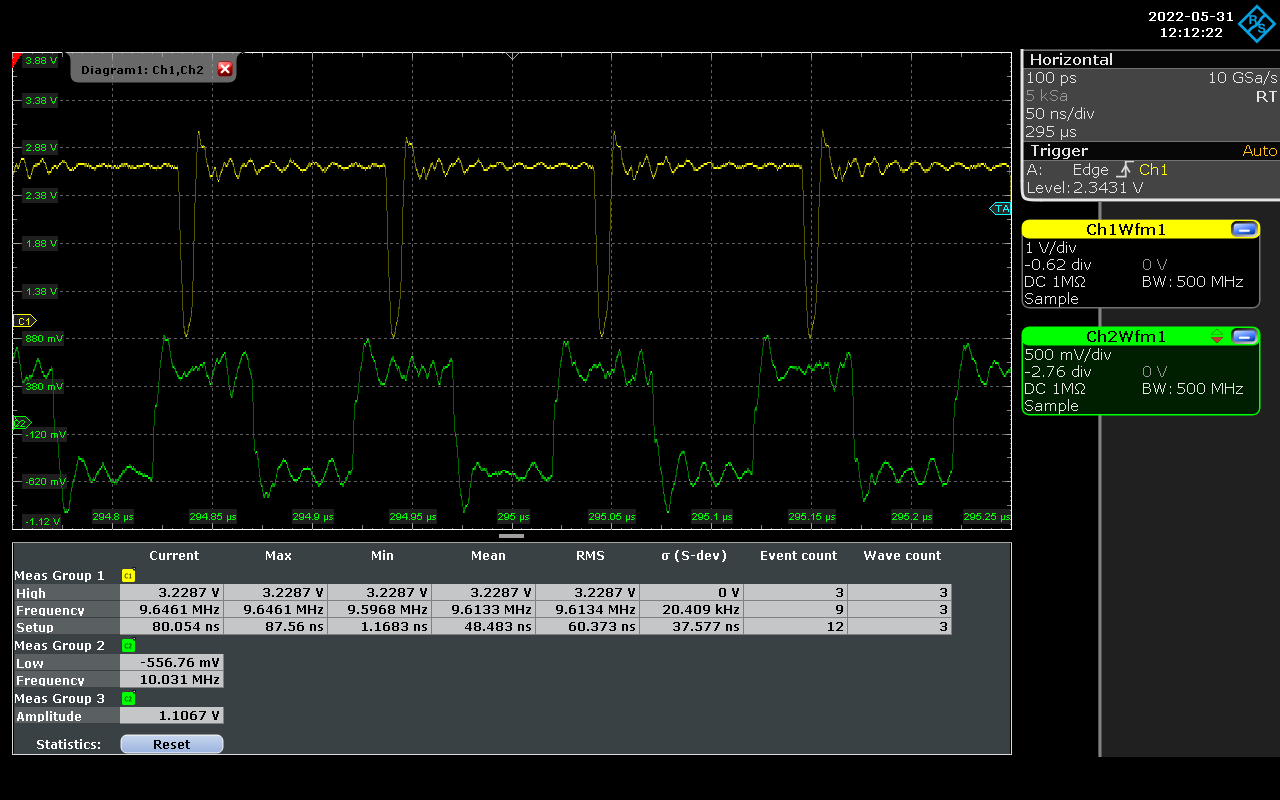
\includegraphics  [scale=0.3] {my_folder/images//stb_10mhz}
	\caption{Генерация строб для 10 Мгц} 
	\label{fig:stb-10mhz}  
\end{figure}

\begin{figure}[ht!] 
	\center
	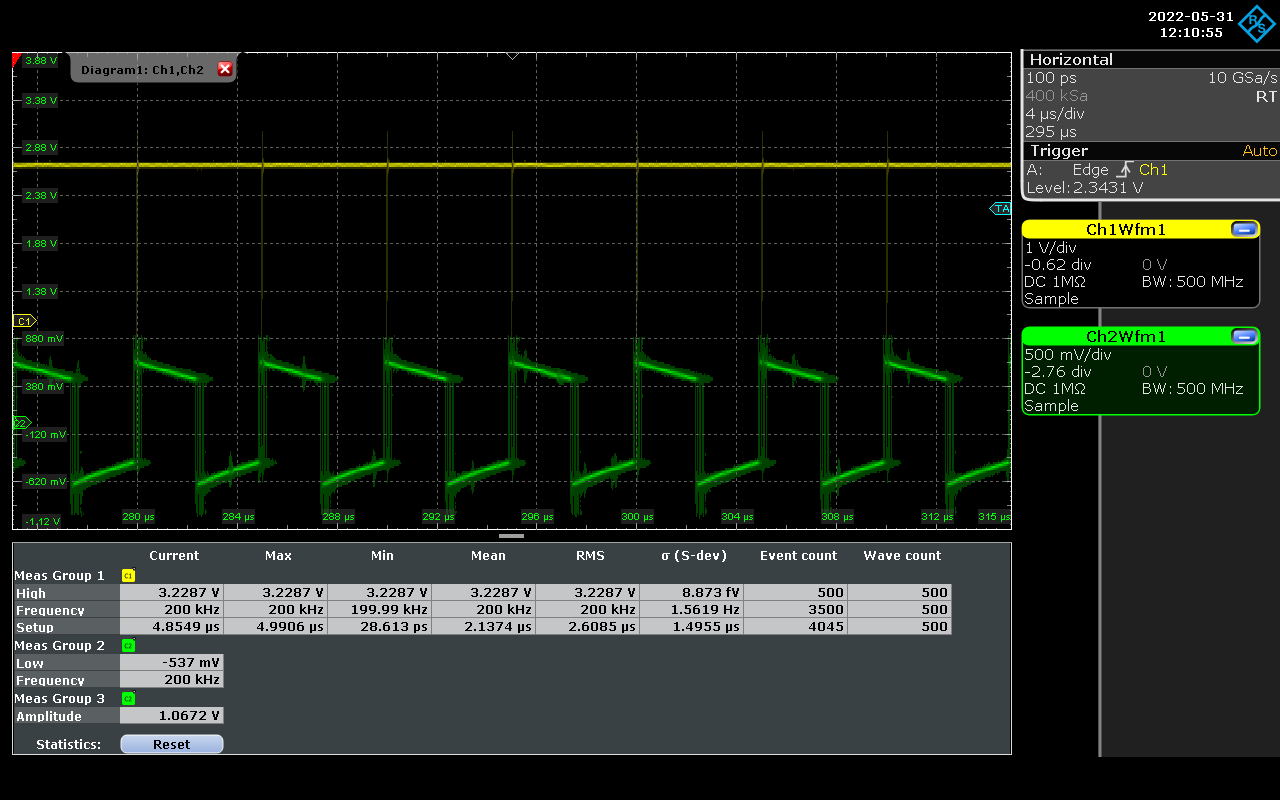
\includegraphics  [scale=0.3] {my_folder/images//stb_200khz}
	\caption{Генерация строб для 200 кГц} 
	\label{fig:stb-200khz}  
\end{figure}

\FloatBarrier

На \firef{fig:stb-10mhz} и \firef{fig:stb-200khz} приведены осциллограммы генерации строб для 10 МГц и 200 кГц.
Видно, что точно определить не кратную частоту невозможно -- при генерации получается стробы с частотой 9.6 Мгц, а не 10 Мгц.

\subsection{Модуль \emph{ch\_measure\_ctl}}

Данный модуль управляет измерением одного из каналов -- выставляет необходимое пороговое напряжение и задержку, а
затем выставляет запрос на стробу. После прохода стробы, в зависимости от текущего и предыдущего выхода компаратора, принимается решение
о следующем значении задержки и порогового напряжения.

Для ускорения снятия осциллограммы применяется предсказание направления изменения сигнала. Для этого, после нахождения очередной точки,
изменяется только задержка, после чего на основании выхода компаратора принимается решение -- измеряемый сигнал нарастает или уменьшается.

\begin{figure}[ht!] 
	\center
	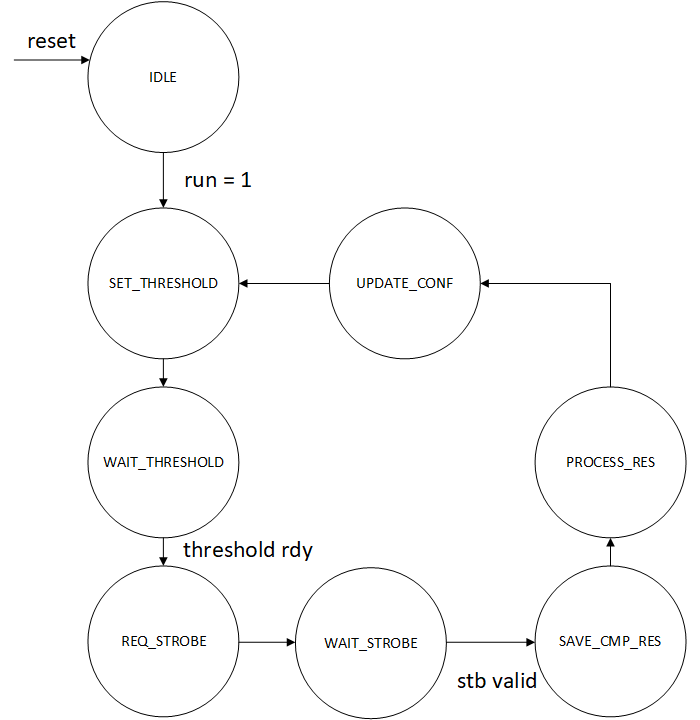
\includegraphics  [scale=0.7] {my_folder/images//ch_ctl}
	\caption{Конечный автомат модуля \emph{ch\_measure\_ctl}} 
	\label{fig:ch-ctl-fsm}  
\end{figure}

\FloatBarrier

На \firef{fig:ch-ctl-fsm} представлен конечный автомат описываемого модуля.

\noindent
\begin{itemize}[label={}]
	\item IDLE -- состояние покоя 
	\item SET\_THRESHOLD -- отправление запроса на установку порогового напряжения ($ \emph{threshold\_wre\_o} = 1 $)
	\item WAIT\_THRESHOLD -- ожидание установки порогового напряжения ($ \emph{threshold\_rdy\_i} == 1 $)
	\item REQ\_STROBE -- установка запроса на стробу ($ \emph{stb\_req\_o} = 1 $)
	\item WAIT\_STROBE -- ожидание прохода стробы ($ \emph{stb\_valid\_i} == 1 $)
	\item SAVE\_CMP\_RES -- обновление текущего и предыдущего выхода компаратора
	\item PROCESS\_RES -- принятие решения о статусе поиска точки (определение направления поиска или поиск точки)
					и о выборе направления поиска
	\item UPDATE\_CONF -- обновление регистров с текущей задержкой и пороговым напряжением на основании принятого ранее решения\\
\end{itemize}

В состоянии PROCESS\_RES, в зависимости от выхода компаратора переключаются два других конечных автомата, отвечающих за статус поиска точки и направления поиска.

На \firef{fig:p-find} приведён пример снятия осциллограммы сигнала.

\begin{figure}[ht!] 
	\center
	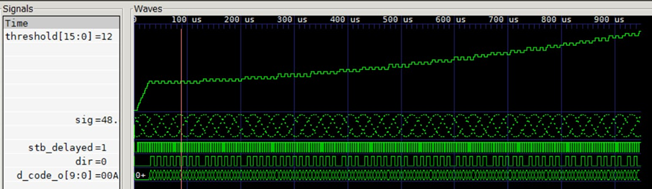
\includegraphics  {my_folder/images//p_find}
	\caption{Пример снятия осциллограммы с угадыванием направления изменения сигнала} 
	\label{fig:p-find}  
\end{figure}

\subsection{Программный интерфейс}

Управление измерительным модулем осуществляется через memory-mapped регистры ( \firef{fig:stb-reg}, \firef{fig:delta-reg},
\firef{fig:thr-reg}, \firef{fig:mu-ctl-reg}, \firef{fig:mu-p-reg}
).

\begin{register}{H}{STB\_GEN\_CTL}{}% name=example
\label{example}%
\regfield{}{29}{3}{{reserved}}%
\regfield{clk\_sel}{1}{2}{{1/0}}%
\regfield{mux}{1}{1}{{1/0}}%
\regfield{run}{1}{0}{{1/0}}%
\reglabel{(w)} \regnewline%

\regfield{}{29}{3}{{reserved}}%
\regfield{clk\_sel}{1}{2}{{1/0}}%
\regfield{mux}{1}{1}{{1/0}}%
\regfield{rdy}{1}{0}{{1/0}}%
\reglabel{(r)}\regnewline%
\end{register}

\begin{register}{H}{STB\_GEN\_PERIOD}{}% name=example
\label{example}%
\regfield{period}{32}{0}{{read only}}%
\reglabel{(r)} \regnewline%
\end{register}

\begin{figure}[ht!] 
	\center
	
\includegraphics  {my_folder/images//blank}
	\caption{Регистры для управления модулем \emph{stb\_gen}} 
	\label{fig:stb-reg}  
\end{figure}

\noindent
\begin{itemize}[label={}]
	\item \textbf{run} -- запись 1 начинает измерение частоты входного сигнала
	\item \textbf{mux} -- выбор канала для измерения (0 -- первый канал, 1 -- второй)
	\item \textbf{clk\_sel} -- выбор источника тактового сигнала для генерации строб (0 -- внутренний, 1 -- внешний)
	\item \textbf{rdy} -- 1 при окончании измерения
	\item \textbf{period} -- измеренное значение периода (кол-во отсчётов счётчика)\\
\end{itemize}

\begin{register}{H}{CH\_CTL\_DELTA\_REG}{}% name=example
\label{example}%
\regfield{}{7}{26}{{reserved}}%
\regfield{delay delta}{10}{16}{{default: 0x01}}%
\regfield{threshold delta}{16}{0}{{default: 0x01}}%
\reglabel{(r/w)} \regnewline%

\end{register}


\begin{figure}[ht!] 
	\center
	
\includegraphics  {my_folder/images//blank}
	\caption{Регистр для задания параметров измерения} 
	\label{fig:delta-reg}  
\end{figure}
\FloatBarrier

\noindent
\begin{itemize}[label={}]
	\item \textbf{threshold delta} -- шаг изменения порогового напряжения (разрешение по оси OY)
	\item \textbf{delay delta} -- шаг изменения задержки (разрешение по оси OX)\\
\end{itemize}


\begin{register}{H}{W\_THRESHOLD}{}% name=example
\label{example}%
\regfield{}{30}{2}{{reserved}}%
\regfield{dac2 rdy}{1}{1}{{1/0}}%
\regfield{dac1 rdy}{1}{0}{{1/0}}%
\reglabel{(r)} \regnewline%

\regfield{}{16}{16}{{reserved}}%
\regfield{threshold}{16}{0}{{}}%
\reglabel{(w)}\regnewline%
\end{register}

\begin{figure}[ht!] 
	\center
	
\includegraphics  {my_folder/images//blank}
	\caption{Регистр для установки порогового напряжения} 
	\label{fig:thr-reg}  
\end{figure}
\FloatBarrier
\noindent
\begin{itemize}[label={}]
	\item \textbf{dac1/2 rdy} -- ЦАП на первом/втором канале установил указанное напряжение
	\item \textbf{threshold} -- запись в это поле устанавливает заданное напряжение на оба канала\\
\end{itemize}
\newpage
\FloatBarrier

\begin{register}{H}{MU\_CTL\_1/2}{}% name=example
\label{example}%
\regfield{}{31}{1}{{reserved}}%
\regfield{run}{1}{0}{{1/0}}%
\reglabel{(r/w)} \regnewline%
\end{register}

\begin{figure}[ht!] 
	\center
	
\includegraphics  {my_folder/images//blank}
	\caption{Регистр для управление измерением канала} 
	\label{fig:mu-ctl-reg}  
\end{figure}
\FloatBarrier
\begin{itemize}[label={}]
	\item \textbf{run} -- запись 1 начинает измерение\\
\end{itemize}


\begin{register}{H}{MU\_CH\_1/2\_VAL}{}% name=example
\label{example}%
\regfield{}{15}{17}{{reserved}}%
\regfield{measured point}{16}{1}{{}}%
\regfield{valid}{1}{0}{{1/0}}%
\reglabel{(r)} \regnewline%
\end{register}

\begin{figure}[ht!] 
	\center
	
\includegraphics  {my_folder/images//blank}
	\caption{Регистр для чтения измеренных значений} 
	\label{fig:mu-p-reg}  
\end{figure}
\FloatBarrier
\begin{itemize}[label={}]
	\item \textbf{measured point} -- значение измеренной точки
	\item \textbf{valid} -- 1 если FIFO не пустое и прочитано измеренное значение\\
\end{itemize}

\FloatBarrier


\newpage           	 % Глава 3
%\chapter{Разработка программной части управляющего устройства}

Программная часть состоит из двух компонентов: загрузчика (\emph{/bootloader/}) и управляющей программы (\emph{/firmware/}).

Загрузчик необходим для обновления прошивки на FLASH памяти внутри калибратора. При запуске устройства загрузчик проверяет
включен ли переключатель на печатной плате калибратора, если нет, то исполнение передаётся управляющей программе.

Все измерения проводятся аппаратно, процессорное ядро используется только для подачи команд на проведение измерений и
взаимодействия с устройством верхнего уровня. На данный момент интеграция с инфраструктурой White Rabbit только планируется,
поэтому все результаты выводятся через последовательный порт в консоль подключенного к калибратору ПК.



\newpage           	 % Глава 3
\ContinueChapterEnd % завершить размещение глав <<подряд>>
%% Завершение основной части

%\chapter*{Заключение} \label{ch-conclusion}
\addcontentsline{toc}{chapter}{Заключение}	% в оглавление 

В результате работы получено управляющее устройство для калибратора субнаносекундной синхронизации.
Поставленные задачи: портирование под целевую ПЛИС и интеграция в СнК открытых модулей, создание
модулей для проведения измерений при помощи стробирования, написание и отладка встраиваемого программного обеспечения -- выполнены в полном объёме.\\

\noindent В процессе работы были освоены:
\begin{itemize}
	\item Маршрут проектирования на ПЛИС пр-ва Gowin Semiconductor
	\item Открытая шина для СнК Wishbone и разработка ведомых устройств для неё
	\item Применение открытого синтезируемого ядра на базе архитектуры RISC-V -- PicoRV32
	\item Проектирование и реализация СнК на основе открытых модулей
	\item Конфигурация компилятора и компоновщика под используемую ISA и СнК\\
\end{itemize}

На данный момент калибратор находится на этапе отладки, планируется вторая ревизия платы с исправлением ошибок, найденных в ходе отладки.
В планах на дальнейшую разработку имеется доработка прошивки, связанная с:
\begin{itemize}
	\item Улучшением метода определения частоты измеряемого сигнала и генерации строб
	\item Доработкой алгоритма и реализации снятия осциллограммы
	\item Добавлением интеграции в инфраструктуру White Rabbit\\
\end{itemize}

Также планируется проведение процедуры калибровки разработанного устройства, что позволит повысить точность проводимых измерений.
        	 % Заключение

%% Наличие следующих перечней не исключает расшифровку сокращения и условного обозначения при первом упоминании в тексте!
%\chapter*{Список сокращений и условных обозначений}             % Заголовок
\addcontentsline{toc}{chapter}{Список сокращений и условных обозначений}  % Добавляем его в оглавление
\noindent
\addtocounter{table}{-1}% Нужно откатить на единицу счетчик номеров таблиц, так как следующая таблица сделана для удобства представления информации по ГОСТ
%\begin{longtabu} to \dimexpr \textwidth-5\tabcolsep {r X}
\begin{longtabu} to \textwidth {r X} % Таблицу не прорисовываем!
% Жирное начертание для математических символов может иметь
% дополнительный смысл, поэтому они приводятся как в тексте
% диссертации
\textbf{WoS} & Web of Science. \\
\textbf{ВКР}  & Выпускная квалификационная работа. \\

\end{longtabu}
		         % Необязательная рубрика! Список сокращений и условных обозначений

%\input{my_folder/dictionary}    		 % Необязательная рубрика! Словарь терминов
% По порядку после Списка сокращений и условных обозначений, если есть.	


\clearpage                                  % В том числе гарантирует, что список литературы в оглавлении будет с правильным номером страницы
\urlstyle{rm}                               % ссылки URL обычным шрифтом
\chapter*{Список использованных источников}
\label{references}
\addcontentsline{toc}{chapter}{Список использованных источников}	% в оглавление 
\printbibliography[env=SSTfirst] 
\noindent
1. Пешков Д.В., Михайловский В.С. Калибрующее устройство для средств высокоточной синхронизации распределённых систем потоковой обработки данных // Экономика и Индустрия 5.0 в условиях новой реальности (ИНПРОМ-2022): сборник трудов Всероссийской научно-практической конференции с зарубежным участием 28-30 апреля 2022. - СПб.: ПОЛИТЕХ-ПРЕСС, 2022. - С. 680-684.\\
2. ADCMP582BCPZ Datasheet [Электронный ресурс] // Analog Devices URL: \url{https://www.analog.com/media/en/technical-documentation/data-sheets/adcmp580\_581\_582.pdf} (дата обращения: 16.06.2022).\\
3. AD5662BRMZ Datasheet [Электронный ресурс] // Analog Devices URL: \url{https://www.analog.com/media/en/technical-documentation/data-sheets/ad5662.pdf} (дата обращения: 16.06.2022).\\
4. Another Wishbone (or even AXI-lite) Controlled UART [Электронный ресурс] // Github URL: \url{https://github.com/ZipCPU/wbuart32} (дата обращения: 16.06.2022).\\
5. FT2232HL Datasheet [Электронный ресурс] // FTDI Chip URL: \url{https://www.ftdichip.com/Support/Documents/DataSheets/ICs/DS\_FT2232H.pdf} (дата обращения: 16.06.2022).\\
6. Grzegorz Daniluk. White Rabbit calibration procedure [Электронный ресурс] // CERN BE-CO-HT URL: \url{https://www.ohwr.org/project/white-rabbit/uploads/76cdbdbadccc9d6c54d5caf246550fbf/WR\_Calibration-v1.1-20151109.pdf} (дата обращения: 16.06.2022).\\
7. GW1N series of FPGA Products Data Sheet DS100-2.7.1E [Электронный ресурс] // GOWIN Semiconductor Corp. URL: \url{https://gowinsemi.com/upload/database\_doc/1752/document/6296db1b68af5.pdf} (дата обращения: 16.06.2022).\\
8. GowinSynthesis User Guide [Электронный ресурс] // GOWIN Semiconductor Corp. URL: \url{http://cdn.gowinsemi.com.cn/SUG550E.pdf} (дата обращения: 16.06.2022).\\
9. Gowin FPGA Primitive User Guide [Электронный ресурс] // GOWIN Semiconductor Corp. URL: \url{https://www.gowinsemi.com/upload/database\_doc/39/document/5bfcff2ce0b72.pdf} (дата обращения: 16.06.2022).\\
10. OpenCores Free and Open Source gateware IP cores [Электронный ресурс] // OpenCores URL: \url{https://opencores.org/} (дата обращения: 16.06.2022).\\
11. PicoRV32 - A Size-Optimized RISC-V CPU [Электронный ресурс] // Github URL: \url{https://github.com/YosysHQ/picorv32} (дата обращения: 16.06.2022).\\
12. SY100EP196V Datasheet [Электронный ресурс] // Microchip URL: \url{https://ww1.microchip.com/downloads/aemDocuments/documents/TCG/ProductDocuments/DataSheets/SY100EP196V-3.3V-5V-2.5GHz-Programmable-Delay-Chip-with-Fine-Tune-Control-DS20006520A.pdf} (дата обращения: 16.06.2022).\\
13. WB2AXIP: Bus interconnects, bridges, and other components [Электронный ресурс] // Github URL: \url{https://github.com/ZipCPU/wb2axip} (дата обращения: 16.06.2022).\\
14. WISHBONE System-on-Chip (SoC)Interconnection Architecture for Portable IP Cores [Электронный ресурс] // OpenCores URL: \url{https://cdn.opencores.org/downloads/wbspec\_b4.pdf} (дата обращения: 16.06.2022). \\
		     % Список литературы

% Здесь можно поместить список иллюстративного материала

\appendix % не редактировать / keep unmodified


\chapter{Исходные коды измерительного модуля}\label{appendix-MikTeX-TexStudio}							% Заголовок
%\addcontentsline{toc}{chapter}{Second call for chapters to participate in the book Machine learning in analysis of biomedical and socio-economic data}	% Добавляем его в оглавление

\begin{flushright}
Листинг П1.1. \emph{stb\_gen.sv}
\end{flushright}

\begin{lstlisting}
module stb_gen #(
	parameter OFFSET = 20,
	parameter T_CNT_WIDTH = 32
) (
	input wire clk_i,
	input wire arst_i,

	input wire sig_i,

	output logic err_o,
	output logic rdy_o,
	output logic stb_o,
	output logic [T_CNT_WIDTH-1:0] stb_period_o,

	input  logic stb_req_i,
	output logic stb_valid_o,
	output logic debug_stb_o
);
	// localparam T_CNT_WIDTH 			= 32;
	localparam ZERO_HOLD_CYCLES 	= 2;

	logic int_stb = 0;
	assign debug_stb_o = int_stb;

	logic sig_synced;

	//stb req interface

	logic stb_oe; // stb_oe == 1 blocks strobe generation

	assign stb_o = (rdy_o ? int_stb | stb_oe : int_stb);	

	assign stb_valid_o = stb_oe & rdy_o;

	logic prev_stb_req;

	always_ff @(posedge clk_i) prev_stb_req <= stb_req_i;

	logic req_posedge;
	assign req_posedge = ~prev_stb_req & stb_req_i;

	logic is_zero_hold_start;
	logic is_stb_end;

	always_ff @(posedge clk_i, negedge arst_i) begin
		if (~arst_i) begin
			stb_oe = 0;
		end else begin
			casex ({req_posedge, is_stb_end})			
				2'bx1:  stb_oe <= 1;
				2'b1x:	stb_oe <= 0;
			endcase
		end
	end

	sync_ff #(
		.WIDTH (1),
		.STAGES(2)
	) sig_i_sync_ff_inst (
		.clk_i (clk_i),
		.data_i(sig_i),
		.data_o(sig_synced)
	);

	logic prev_sig; //edge detect

	always_ff @(posedge clk_i) begin
		prev_sig <= sig_synced;
	end

	logic sig_posedge;
	assign sig_posedge = sig_synced & ~prev_sig;

	typedef enum logic[8:0] { 
		FIND_EDGE_1 		= 9'b000000001, 
		FIND_EDGE_2 		= 9'b000000010,
		WRITE_START 		= 9'b000000100,
		FIND_EDGE_3 		= 9'b000001000, 
		WRITE_END			= 9'b000010000,
		COUNT_PERIOD 		= 9'b000100000, 
		WAIT_COUNT_PERIOD 	= 9'b001000000,
		COUNT_STROBE 		= 9'b010000000,
		WAIT_STB_END 		= 9'b100000000
	} stb_gen_state;

	stb_gen_state state = FIND_EDGE_1;

	logic [T_CNT_WIDTH-1 : 0] t_cnt /* synthesis syn_keep=1 syn_preserve=1 syn_ramstyle="registers" */;
	logic [T_CNT_WIDTH-1 : 0] t_start;
	logic [T_CNT_WIDTH-1 : 0] t_end;
	stb_gen_state next_state;


	logic count_zero_hold_begin, zero_hold_begin_valid;
	logic count_stb_end, stb_end_valid;

	assign count_zero_hold_begin = (state == COUNT_STROBE ? 1 : 0);
	assign count_stb_end = (state == COUNT_STROBE ? 1 : 0);

	always_comb begin
		unique case (state) /* sythesis parallel_case*/
			FIND_EDGE_1:			if (sig_posedge) next_state = FIND_EDGE_2;
									else next_state = state;
			FIND_EDGE_2:			if (sig_posedge) next_state = WRITE_START;
									else next_state = state;
			WRITE_START:			next_state = FIND_EDGE_3;
			FIND_EDGE_3:			if (sig_posedge) next_state = WRITE_END;
									else next_state = state;
			WRITE_END:				next_state = COUNT_PERIOD;
			COUNT_PERIOD:			next_state = WAIT_COUNT_PERIOD;
			WAIT_COUNT_PERIOD:		next_state = COUNT_STROBE;
			COUNT_STROBE:			next_state = WAIT_STB_END;
			WAIT_STB_END:			if (is_stb_end) next_state = COUNT_STROBE;
									else next_state = state;
			default:				next_state = state;
		endcase
	end

	always_ff @(posedge clk_i, negedge arst_i) begin
		if (~arst_i) begin
			state = FIND_EDGE_1;
		end else begin
			state <= next_state;
		end
	end

	logic [T_CNT_WIDTH-1:0] adder_zero_hold_res;
	logic [T_CNT_WIDTH-1:0] adder_stb_end_res;

	always_ff @(posedge clk_i) begin
		stb_period_o <= (state == COUNT_PERIOD ? t_end - t_start : stb_period_o);
	end

	localparam MAGIC_CONST = 3;

	logic [T_CNT_WIDTH-1:0] period_minus_zero_hold;
	always_ff @(posedge clk_i) period_minus_zero_hold <= stb_period_o - (ZERO_HOLD_CYCLES+MAGIC_CONST); //magic constat due to computation pipeline

	two_cycle_32_adder adder_zero_hold_begin (
		.clk_i 	(clk_i),
		.a_i	(t_cnt),
		.b_i	(period_minus_zero_hold),
		.valid_i(count_zero_hold_begin),
		.valid_o(zero_hold_begin_valid),
		.res_o	(adder_zero_hold_res)
	);

	two_cycle_32_adder adder_stb_end (
		.clk_i 	(clk_i),
		.a_i	(t_cnt),
		.b_i	(stb_period_o - MAGIC_CONST), //magic constat due to computation pipeline
		.valid_i(count_stb_end),
		.valid_o(stb_end_valid),
		.res_o	(adder_stb_end_res)
	);

	logic [T_CNT_WIDTH-1:0] latched_zero_hold_res;
	logic [T_CNT_WIDTH-1:0] latched_stb_end_res;

	always_ff @(posedge clk_i) latched_zero_hold_res <= (zero_hold_begin_valid ? adder_zero_hold_res : latched_zero_hold_res);
	always_ff @(posedge clk_i) latched_stb_end_res <= (stb_end_valid ? adder_stb_end_res : latched_stb_end_res);

 
	logic is_zero_hold_start_lo;
	logic is_zero_hold_start_hi;
	logic is_stb_end_lo;
	logic is_stb_end_hi;

	always_ff @(posedge clk_i) is_zero_hold_start_lo <=  ~|(t_cnt[15:0] ^ latched_zero_hold_res[15:0]);  //t_cnt == latched_zero_hold_res;
	always_ff @(posedge clk_i) is_zero_hold_start_hi <=  ~|(t_cnt[31:16] ^ latched_zero_hold_res[31:16]);  //t_cnt == latched_zero_hold_res;
	always_ff @(posedge clk_i) is_zero_hold_start <= is_zero_hold_start_lo & is_zero_hold_start_hi; 

	always_ff @(posedge clk_i) is_stb_end_lo <=  ~|(t_cnt[15:0] ^ latched_stb_end_res[15:0]);  //t_cnt == latched_zero_hold_res;
	always_ff @(posedge clk_i) is_stb_end_hi <=  ~|(t_cnt[31:16] ^ latched_stb_end_res[31:16]);  //t_cnt == latched_zero_hold_res;
	always_ff @(posedge clk_i) is_stb_end <= is_stb_end_hi & is_stb_end_lo; 

	always_ff @(posedge clk_i, negedge arst_i) begin
		if (~arst_i) begin
			int_stb = 0;
		end else begin
			case (1) 
				is_zero_hold_start: int_stb <= 0;
				is_stb_end:			int_stb <= 1;
				default:			int_stb <= int_stb;
			endcase
		end
	end

	always_ff @(posedge clk_i, negedge arst_i) begin
		if (~arst_i) rdy_o = 0;
		else rdy_o <= (state == COUNT_STROBE ? 1 : rdy_o);
	end

	always_ff @(posedge clk_i) begin
		err_o <= (state == FIND_EDGE_1 ? 0 : err_o);
	end

	always_ff @(posedge clk_i) t_end <= (state == WRITE_END ? t_cnt : t_end);

	always_ff @(posedge clk_i) t_start <= (state == WRITE_START ? t_cnt : t_start);

	// pipelined counter

	logic [T_CNT_WIDTH/2-1 : 0] high_bytes = 0 			/* synthesis syn_keep=1 syn_preserve=1 syn_ramstyle="registers" */;
	logic [T_CNT_WIDTH/2-1 : 0] latched_low_bytes = 0 	/* synthesis syn_keep=1 syn_preserve=1 syn_ramstyle="registers" */;
	logic [T_CNT_WIDTH/2-1 : 0] low_bytes = 0 			/* synthesis syn_keep=1 syn_preserve=1 syn_ramstyle="registers" */;
	logic [T_CNT_WIDTH/2-1 : 0] low_bytes_plus_1;
	logic carry;

	assign {carry, low_bytes_plus_1} = low_bytes + 1;

	//incrementing low bytes
	always_ff @(posedge clk_i, negedge arst_i) 
		if (~arst_i) low_bytes = 0;
		else low_bytes <= low_bytes_plus_1;

	//latching low bytes for 1 cycle
	always_ff @(posedge clk_i, negedge arst_i) 
		if (~arst_i) latched_low_bytes = 0;
		else latched_low_bytes <= low_bytes;

	logic latched_carry = 0;

	//latching carry
	always_ff @(posedge clk_i, negedge arst_i) 
		if (~arst_i) latched_carry = 0;
		else latched_carry <= carry;

	//adding latched carry to high bytes
	always_ff @(posedge clk_i, negedge arst_i)
		if (~arst_i) high_bytes = 0;
		else high_bytes <= high_bytes + latched_carry;

	//seting t_cnt
	always_ff @(posedge clk_i, negedge arst_i) 
		if (~arst_i) t_cnt = 0;
		else t_cnt <= {high_bytes, latched_low_bytes};

endmodule
\end{lstlisting}

\begin{flushright}
Листинг П1.2. \emph{two\_cycle\_32\_adder.sv}
\end{flushright}

\begin{lstlisting}
module two_cycle_32_adder (
    input logic clk_i,
    input logic [31:0] a_i,
    input logic [31:0] b_i,
    input logic valid_i,

    output logic valid_o,
    output logic [31:0] res_o
);
    
    logic [31:0] a, b;

    always_ff @(posedge clk_i) begin
        a <= (valid_i ? a_i : a);
        b <= (valid_i ? b_i : b);
    end

    enum logic[2:0] {
        IDLE            = 3'b001, 
        FIRST_STAGE     = 3'b010, 
        SECOND_STAGE    = 3'b100
    } state = IDLE, next_state;

    always_ff @(posedge clk_i) state <= next_state;
  
    logic [1:0] valid;
    integer i;
    always_ff @(posedge clk_i) begin
        valid[0] <= valid_i;
        for (i = 1; i <= 1; i = i +1 ) valid[i] <= valid[i-1];
        valid_o <= valid[1];
    end


    always_comb begin
        next_state = state;
        case (state)
            IDLE: if (valid_i) next_state = FIRST_STAGE;
            FIRST_STAGE: next_state = SECOND_STAGE;
            SECOND_STAGE: next_state = IDLE;
        endcase
    end

    logic carry;

    always_ff @(posedge clk_i) begin
        case (state) 
            FIRST_STAGE: {carry, res_o[15:0]} <= a[15:0] + b[15:0];
            default: {carry, res_o[15:0]} <= {carry, res_o[15:0]};
        endcase
        case (state)
            SECOND_STAGE: res_o[31:16] <= a[31:16] + b[31:16] + carry;
            default: res_o[31:16] <= res_o[31:16];
        endcase
    end

endmodule
\end{lstlisting}

\begin{flushright}
Листинг П1.3. \emph{sc\_fifo.sv}
\end{flushright}

\begin{lstlisting}
module sc_fifo #(
    parameter LGFLEN = 10,
    parameter WIDTH = 32
) (
    input logic     clk_i,
    input logic     arstn_i,

    input logic [WIDTH-1:0] data_i,
    input logic             wre_i,

    output logic [WIDTH-1:0] data_o,
    input  logic             re_i,
    output logic             n_empty_o
);

    logic [WIDTH-1:0] cyc_buf [int'($pow(2, LGFLEN)-1):0];

    logic [LGFLEN-1:0] r_addr, w_addr;

    assign n_empty_o = (r_addr != w_addr);
    assign data_o = cyc_buf[r_addr];

    always_ff @(posedge clk_i/*, negedge arstn_i*/) begin : w_addr_ff
        if (~arstn_i) begin
            w_addr = 0;
        end else begin
            if (wre_i) begin
                w_addr <= w_addr + 1;
            end
        end
    end

    always_ff @(posedge clk_i/*, negedge arstn_i*/) begin : r_addr_ff
        if (~arstn_i) begin
            r_addr = 0;
        end else begin
            if (re_i & n_empty_o) begin
                r_addr <= r_addr + 1;
            end
        end
    end

    always_ff @(posedge clk_i) begin
        if (wre_i) begin
            cyc_buf[w_addr] <= data_i;
        end
    end

endmodule
\end{lstlisting}

\begin{flushright}
Листинг П1.4. \emph{ch\_measure\_ctl.sv}
\end{flushright}

\begin{lstlisting}
module ch_measure_ctl #(
	parameter DEFAULT_THRESHOLD_DELTA = 1,
	parameter DEFAULT_D_CODE_DELTA = 1    
) (
	input logic clk_i,
	input logic arst_i,

	//stb request interface
	output logic stb_req_o,
	input  logic stb_valid_i,

	//CMP input
	input logic cmp_out_i,

	//control threshold and delay delta
	input logic [15:0] threshold_delta_i,
	input logic [9:0] d_code_delta_i,

	//dac (threshold) output
	output logic [15:0] threshold_o,
	output logic threshold_wre_o,
	input logic threshold_rdy_i,

	//delay line
	output logic [9:0] d_code_o,

	//ctl
	input logic run_i,

	//TODO output measured value
	output logic point_rdy_o
);

	enum logic[7:0] { 
		IDLE 		        = 8'b00000001,
		SET_THRESHOLD 		= 8'b00000010,
		WAIT_THRESHOLD 		= 8'b00000100,
		REQ_STROBE 			= 8'b00001000,
		WAIT_STROBE			= 8'b00010000,
		SAVE_CMP_RES		= 8'b00100000,
		PROCESS_RES			= 8'b01000000,
		UPDATE_CONF			= 8'b10000000
	} ctl_state, next_ctl_state;

	enum logic [1:0] {
		DIR_UP		= 2'b01,
		DIR_DOWN	= 2'b10
	} threshold_dir;

	enum logic [1:0] {
		FIND_DIR	= 2'b01,
		FIND_POINT	= 2'b10
	} point_state, next_point_state;

	logic cur_cmp_out, prev_cmp_out;

	always_comb begin : next_ctl_state_comb
		if (~run_i) begin
			next_ctl_state = IDLE;
		end else begin
			case (ctl_state)
				IDLE:   			next_ctl_state = SET_THRESHOLD;
				SET_THRESHOLD:		next_ctl_state = WAIT_THRESHOLD;
				WAIT_THRESHOLD:		if (threshold_rdy_i) next_ctl_state = REQ_STROBE;
									else next_ctl_state = ctl_state;
				REQ_STROBE:			next_ctl_state = WAIT_STROBE;	
				WAIT_STROBE:		if (stb_valid_i) next_ctl_state = SAVE_CMP_RES;
									else next_ctl_state = ctl_state;

				SAVE_CMP_RES:		next_ctl_state = PROCESS_RES;
				PROCESS_RES:		next_ctl_state = UPDATE_CONF;
				UPDATE_CONF:		next_ctl_state = SET_THRESHOLD;

			endcase
		end
	end

	always_comb begin : next_point_state_comb
		if (ctl_state == PROCESS_RES) begin
			case (point_state) /* synthesis full_case */
				FIND_POINT: if (cur_cmp_out != prev_cmp_out) next_point_state = FIND_DIR;
							else next_point_state = point_state;
				FIND_DIR:	next_point_state = FIND_POINT;
			endcase
		end else begin
			next_point_state = point_state;
		end
	end

	always_ff @(posedge clk_i, negedge arst_i) begin
		if (~arst_i) begin
			cur_cmp_out = 1;
		end else if (ctl_state == SAVE_CMP_RES) begin
			cur_cmp_out <= cmp_out_i;
			prev_cmp_out <= cur_cmp_out;
		end
	end

	always_ff @(posedge clk_i, negedge arst_i) begin : ctl_state_ff
		if (~arst_i) begin
			ctl_state = IDLE;
		end else begin
			ctl_state <= next_ctl_state;
		end
	end

	logic [15:0] next_threshold;
	logic [9:0]	 next_d_code;

	always_comb begin : next_threshold_comb
		case (ctl_state)
			IDLE:			next_threshold = 0;
			UPDATE_CONF:	if (point_state == FIND_POINT) begin
								case (threshold_dir) /* synthesis full_case */
									DIR_UP: 	next_threshold = threshold_o + threshold_delta_i;
									DIR_DOWN:	next_threshold = threshold_o - threshold_delta_i;	
								endcase
							end else begin
								next_threshold = threshold_o;
							end
			default:		next_threshold = threshold_o;
		endcase
	end

	always_comb begin : next_d_code_comb
		case (ctl_state)
			IDLE:			next_d_code = 0;
			UPDATE_CONF:	if (point_state == FIND_DIR) begin
				   				next_d_code = d_code_o + d_code_delta_i;
							end else begin
								next_d_code = d_code_o;
							end
			default:		next_d_code = d_code_o;
		endcase
	end

	always_ff @(posedge clk_i, negedge arst_i) begin : threshold_ff
		if (~arst_i) begin
			threshold_o = 0;
		end else begin
			threshold_o <= next_threshold;
		end
	end

	always_ff @(posedge clk_i, negedge arst_i) begin : threshold_wre_ff
		if (~arst_i) begin
			threshold_wre_o = 0;
		end else begin
			case (ctl_state)
				SET_THRESHOLD:  threshold_wre_o <= 1;
				default:        threshold_wre_o <= 0; 
			endcase
		end
	end

	always_ff @(posedge clk_i, negedge arst_i) begin : stb_req_ff
		if (~arst_i) begin
			stb_req_o = 0;
		end else begin
			case (ctl_state)
				REQ_STROBE: stb_req_o <= 1;
				default:	stb_req_o <= 0;
			endcase
		end
	end

	always_ff @(posedge clk_i, negedge arst_i) begin : threshold_dir_ff
		if (~arst_i) begin
			threshold_dir = DIR_UP;
		end else begin
			if (ctl_state == PROCESS_RES & point_state == FIND_DIR) begin
				case ({cur_cmp_out, prev_cmp_out})
					2'b10:		threshold_dir <= DIR_DOWN;	
					2'b01:		threshold_dir <= DIR_UP;	
					default: 	threshold_dir <= (threshold_dir == DIR_DOWN ? DIR_UP : DIR_DOWN);
				endcase
			end
		end
	end

	always_ff @(posedge clk_i, negedge arst_i) begin : point_state_ff
		if (~arst_i) begin
			point_state = FIND_POINT;
		end else begin
			point_state <= next_point_state;
		end
	end

	always_ff @(posedge clk_i, negedge arst_i) begin : d_code_ff
		if (~arst_i) begin
			d_code_o = 0;
		end else begin
			d_code_o <= next_d_code;
		end
	end

	always_ff @(posedge clk_i, negedge arst_i) begin : point_rdy_ff
		if (~arst_i) begin
			point_rdy_o = 0;
		end else begin
			if (ctl_state == PROCESS_RES & cur_cmp_out != prev_cmp_out) point_rdy_o <= 1;
			else point_rdy_o <= 0;
		end
	end

endmodule
\end{lstlisting}




\NewPage % начать новое приложение с новой страницы 
			     % Приложение 1

%\chapter{Исходные коды измерительного модуля}\label{appendix-MikTeX-TexStudio}							% Заголовок
%\addcontentsline{toc}{chapter}{Second call for chapters to participate in the book Machine learning in analysis of biomedical and socio-economic data}	% Добавляем его в оглавление

\begin{flushright}
Листинг П2.1. \emph{stb\_gen.sv}
\end{flushright}

\begin{lstlisting}[language=Verilog]
module stb_gen #(
	parameter OFFSET = 20,
	parameter T_CNT_WIDTH = 32
) (
	input wire clk_i,
	input wire arst_i,

	input wire sig_i,

	output logic err_o,
	output logic rdy_o,
	output logic stb_o,
	output logic [T_CNT_WIDTH-1:0] stb_period_o,

	input  logic stb_req_i,
	output logic stb_valid_o,
	output logic debug_stb_o
);
	// localparam T_CNT_WIDTH 			= 32;
	localparam ZERO_HOLD_CYCLES 	= 2;

	logic int_stb = 0;
	assign debug_stb_o = int_stb;

	logic sig_synced;

	//stb req interface

	logic stb_oe; // stb_oe == 1 blocks strobe generation

	assign stb_o = (rdy_o ? int_stb | stb_oe : int_stb);	

	assign stb_valid_o = stb_oe & rdy_o;

	logic prev_stb_req;

	always_ff @(posedge clk_i) prev_stb_req <= stb_req_i;

	logic req_posedge;
	assign req_posedge = ~prev_stb_req & stb_req_i;

	logic is_zero_hold_start;
	logic is_stb_end;

	always_ff @(posedge clk_i, negedge arst_i) begin
		if (~arst_i) begin
			stb_oe = 0;
		end else begin
			casex ({req_posedge, is_stb_end})			
				2'bx1:  stb_oe <= 1;
				2'b1x:	stb_oe <= 0;
			endcase
		end
	end

	sync_ff #(
		.WIDTH (1),
		.STAGES(2)
	) sig_i_sync_ff_inst (
		.clk_i (clk_i),
		.data_i(sig_i),
		.data_o(sig_synced)
	);

	logic prev_sig; //edge detect

	always_ff @(posedge clk_i) begin
		prev_sig <= sig_synced;
	end

	logic sig_posedge;
	assign sig_posedge = sig_synced & ~prev_sig;

	typedef enum logic[8:0] { 
		FIND_EDGE_1 		= 9'b000000001, 
		FIND_EDGE_2 		= 9'b000000010,
		WRITE_START 		= 9'b000000100,
		FIND_EDGE_3 		= 9'b000001000, 
		WRITE_END			= 9'b000010000,
		COUNT_PERIOD 		= 9'b000100000, 
		WAIT_COUNT_PERIOD 	= 9'b001000000,
		COUNT_STROBE 		= 9'b010000000,
		WAIT_STB_END 		= 9'b100000000
	} stb_gen_state;

	stb_gen_state state = FIND_EDGE_1;

	logic [T_CNT_WIDTH-1 : 0] t_cnt /* synthesis syn_keep=1 syn_preserve=1 syn_ramstyle="registers" */;
	logic [T_CNT_WIDTH-1 : 0] t_start;
	logic [T_CNT_WIDTH-1 : 0] t_end;
	stb_gen_state next_state;


	logic count_zero_hold_begin, zero_hold_begin_valid;
	logic count_stb_end, stb_end_valid;

	assign count_zero_hold_begin = (state == COUNT_STROBE ? 1 : 0);
	assign count_stb_end = (state == COUNT_STROBE ? 1 : 0);

	always_comb begin
		unique case (state) /* sythesis parallel_case*/
			FIND_EDGE_1:			if (sig_posedge) next_state = FIND_EDGE_2;
									else next_state = state;
			FIND_EDGE_2:			if (sig_posedge) next_state = WRITE_START;
									else next_state = state;
			WRITE_START:			next_state = FIND_EDGE_3;
			FIND_EDGE_3:			if (sig_posedge) next_state = WRITE_END;
									else next_state = state;
			WRITE_END:				next_state = COUNT_PERIOD;
			COUNT_PERIOD:			next_state = WAIT_COUNT_PERIOD;
			WAIT_COUNT_PERIOD:		next_state = COUNT_STROBE;
			COUNT_STROBE:			next_state = WAIT_STB_END;
			WAIT_STB_END:			if (is_stb_end) next_state = COUNT_STROBE;
									else next_state = state;
			default:				next_state = state;
		endcase
	end

	always_ff @(posedge clk_i, negedge arst_i) begin
		if (~arst_i) begin
			state = FIND_EDGE_1;
		end else begin
			state <= next_state;
		end
	end

	logic [T_CNT_WIDTH-1:0] adder_zero_hold_res;
	logic [T_CNT_WIDTH-1:0] adder_stb_end_res;

	always_ff @(posedge clk_i) begin
		stb_period_o <= (state == COUNT_PERIOD ? t_end - t_start : stb_period_o);
	end

	localparam MAGIC_CONST = 3;

	logic [T_CNT_WIDTH-1:0] period_minus_zero_hold;
	always_ff @(posedge clk_i) period_minus_zero_hold <= stb_period_o - (ZERO_HOLD_CYCLES+MAGIC_CONST); //magic constat due to computation pipeline

	two_cycle_32_adder adder_zero_hold_begin (
		.clk_i 	(clk_i),
		.a_i	(t_cnt),
		.b_i	(period_minus_zero_hold),
		.valid_i(count_zero_hold_begin),
		.valid_o(zero_hold_begin_valid),
		.res_o	(adder_zero_hold_res)
	);

	two_cycle_32_adder adder_stb_end (
		.clk_i 	(clk_i),
		.a_i	(t_cnt),
		.b_i	(stb_period_o - MAGIC_CONST), //magic constat due to computation pipeline
		.valid_i(count_stb_end),
		.valid_o(stb_end_valid),
		.res_o	(adder_stb_end_res)
	);

	logic [T_CNT_WIDTH-1:0] latched_zero_hold_res;
	logic [T_CNT_WIDTH-1:0] latched_stb_end_res;

	always_ff @(posedge clk_i) latched_zero_hold_res <= (zero_hold_begin_valid ? adder_zero_hold_res : latched_zero_hold_res);
	always_ff @(posedge clk_i) latched_stb_end_res <= (stb_end_valid ? adder_stb_end_res : latched_stb_end_res);

 
	logic is_zero_hold_start_lo;
	logic is_zero_hold_start_hi;
	logic is_stb_end_lo;
	logic is_stb_end_hi;

	always_ff @(posedge clk_i) is_zero_hold_start_lo <=  ~|(t_cnt[15:0] ^ latched_zero_hold_res[15:0]);  //t_cnt == latched_zero_hold_res;
	always_ff @(posedge clk_i) is_zero_hold_start_hi <=  ~|(t_cnt[31:16] ^ latched_zero_hold_res[31:16]);  //t_cnt == latched_zero_hold_res;
	always_ff @(posedge clk_i) is_zero_hold_start <= is_zero_hold_start_lo & is_zero_hold_start_hi; 

	always_ff @(posedge clk_i) is_stb_end_lo <=  ~|(t_cnt[15:0] ^ latched_stb_end_res[15:0]);  //t_cnt == latched_zero_hold_res;
	always_ff @(posedge clk_i) is_stb_end_hi <=  ~|(t_cnt[31:16] ^ latched_stb_end_res[31:16]);  //t_cnt == latched_zero_hold_res;
	always_ff @(posedge clk_i) is_stb_end <= is_stb_end_hi & is_stb_end_lo; 

	always_ff @(posedge clk_i, negedge arst_i) begin
		if (~arst_i) begin
			int_stb = 0;
		end else begin
			case (1) 
				is_zero_hold_start: int_stb <= 0;
				is_stb_end:			int_stb <= 1;
				default:			int_stb <= int_stb;
			endcase
		end
	end

	always_ff @(posedge clk_i, negedge arst_i) begin
		if (~arst_i) rdy_o = 0;
		else rdy_o <= (state == COUNT_STROBE ? 1 : rdy_o);
	end

	always_ff @(posedge clk_i) begin
		err_o <= (state == FIND_EDGE_1 ? 0 : err_o);
	end

	always_ff @(posedge clk_i) t_end <= (state == WRITE_END ? t_cnt : t_end);

	always_ff @(posedge clk_i) t_start <= (state == WRITE_START ? t_cnt : t_start);

	// pipelined counter

	logic [T_CNT_WIDTH/2-1 : 0] high_bytes = 0 			/* synthesis syn_keep=1 syn_preserve=1 syn_ramstyle="registers" */;
	logic [T_CNT_WIDTH/2-1 : 0] latched_low_bytes = 0 	/* synthesis syn_keep=1 syn_preserve=1 syn_ramstyle="registers" */;
	logic [T_CNT_WIDTH/2-1 : 0] low_bytes = 0 			/* synthesis syn_keep=1 syn_preserve=1 syn_ramstyle="registers" */;
	logic [T_CNT_WIDTH/2-1 : 0] low_bytes_plus_1;
	logic carry;

	assign {carry, low_bytes_plus_1} = low_bytes + 1;

	//incrementing low bytes
	always_ff @(posedge clk_i, negedge arst_i) 
		if (~arst_i) low_bytes = 0;
		else low_bytes <= low_bytes_plus_1;

	//latching low bytes for 1 cycle
	always_ff @(posedge clk_i, negedge arst_i) 
		if (~arst_i) latched_low_bytes = 0;
		else latched_low_bytes <= low_bytes;

	logic latched_carry = 0;

	//latching carry
	always_ff @(posedge clk_i, negedge arst_i) 
		if (~arst_i) latched_carry = 0;
		else latched_carry <= carry;

	//adding latched carry to high bytes
	always_ff @(posedge clk_i, negedge arst_i)
		if (~arst_i) high_bytes = 0;
		else high_bytes <= high_bytes + latched_carry;

	//seting t_cnt
	always_ff @(posedge clk_i, negedge arst_i) 
		if (~arst_i) t_cnt = 0;
		else t_cnt <= {high_bytes, latched_low_bytes};

endmodule
\end{lstlisting}

\begin{flushright}
Листинг П2.2. \emph{two\_cycle\_32\_adder.sv}
\end{flushright}

\begin{lstlisting}[language=Verilog]
module two_cycle_32_adder (
    input logic clk_i,
    input logic [31:0] a_i,
    input logic [31:0] b_i,
    input logic valid_i,

    output logic valid_o,
    output logic [31:0] res_o
);
    
    logic [31:0] a, b;

    always_ff @(posedge clk_i) begin
        a <= (valid_i ? a_i : a);
        b <= (valid_i ? b_i : b);
    end

    enum logic[2:0] {
        IDLE            = 3'b001, 
        FIRST_STAGE     = 3'b010, 
        SECOND_STAGE    = 3'b100
    } state = IDLE, next_state;

    always_ff @(posedge clk_i) state <= next_state;
  
    logic [1:0] valid;
    integer i;
    always_ff @(posedge clk_i) begin
        valid[0] <= valid_i;
        for (i = 1; i <= 1; i = i +1 ) valid[i] <= valid[i-1];
        valid_o <= valid[1];
    end


    always_comb begin
        next_state = state;
        case (state)
            IDLE: if (valid_i) next_state = FIRST_STAGE;
            FIRST_STAGE: next_state = SECOND_STAGE;
            SECOND_STAGE: next_state = IDLE;
        endcase
    end

    logic carry;

    always_ff @(posedge clk_i) begin
        case (state) 
            FIRST_STAGE: {carry, res_o[15:0]} <= a[15:0] + b[15:0];
            default: {carry, res_o[15:0]} <= {carry, res_o[15:0]};
        endcase
        case (state)
            SECOND_STAGE: res_o[31:16] <= a[31:16] + b[31:16] + carry;
            default: res_o[31:16] <= res_o[31:16];
        endcase
    end

endmodule
\end{lstlisting}

\begin{flushright}
Листинг П2.3. \emph{sc\_fifo.sv}
\end{flushright}

\begin{lstlisting}[language=Verilog]
module sc_fifo #(
    parameter LGFLEN = 10,
    parameter WIDTH = 32
) (
    input logic     clk_i,
    input logic     arstn_i,

    input logic [WIDTH-1:0] data_i,
    input logic             wre_i,

    output logic [WIDTH-1:0] data_o,
    input  logic             re_i,
    output logic             n_empty_o
);

    logic [WIDTH-1:0] cyc_buf [int'($pow(2, LGFLEN)-1):0];

    logic [LGFLEN-1:0] r_addr, w_addr;

    assign n_empty_o = (r_addr != w_addr);
    assign data_o = cyc_buf[r_addr];

    always_ff @(posedge clk_i/*, negedge arstn_i*/) begin : w_addr_ff
        if (~arstn_i) begin
            w_addr = 0;
        end else begin
            if (wre_i) begin
                w_addr <= w_addr + 1;
            end
        end
    end

    always_ff @(posedge clk_i/*, negedge arstn_i*/) begin : r_addr_ff
        if (~arstn_i) begin
            r_addr = 0;
        end else begin
            if (re_i & n_empty_o) begin
                r_addr <= r_addr + 1;
            end
        end
    end

    always_ff @(posedge clk_i) begin
        if (wre_i) begin
            cyc_buf[w_addr] <= data_i;
        end
    end

endmodule
\end{lstlisting}

\begin{flushright}
Листинг П2.4. \emph{ch\_measure\_ctl.sv}
\end{flushright}

\begin{lstlisting}[language=Verilog]
module ch_measure_ctl #(
	parameter DEFAULT_THRESHOLD_DELTA = 1,
	parameter DEFAULT_D_CODE_DELTA = 1    
) (
	input logic clk_i,
	input logic arst_i,

	//stb request interface
	output logic stb_req_o,
	input  logic stb_valid_i,

	//CMP input
	input logic cmp_out_i,

	//control threshold and delay delta
	input logic [15:0] threshold_delta_i,
	input logic [9:0] d_code_delta_i,

	//dac (threshold) output
	output logic [15:0] threshold_o,
	output logic threshold_wre_o,
	input logic threshold_rdy_i,

	//delay line
	output logic [9:0] d_code_o,

	//ctl
	input logic run_i,

	//TODO output measured value
	output logic point_rdy_o
);

	enum logic[7:0] { 
		IDLE 		        = 8'b00000001,
		SET_THRESHOLD 		= 8'b00000010,
		WAIT_THRESHOLD 		= 8'b00000100,
		REQ_STROBE 			= 8'b00001000,
		WAIT_STROBE			= 8'b00010000,
		SAVE_CMP_RES		= 8'b00100000,
		PROCESS_RES			= 8'b01000000,
		UPDATE_CONF			= 8'b10000000
	} ctl_state, next_ctl_state;

	enum logic [1:0] {
		DIR_UP		= 2'b01,
		DIR_DOWN	= 2'b10
	} threshold_dir;

	enum logic [1:0] {
		FIND_DIR	= 2'b01,
		FIND_POINT	= 2'b10
	} point_state, next_point_state;

	logic cur_cmp_out, prev_cmp_out;

	always_comb begin : next_ctl_state_comb
		if (~run_i) begin
			next_ctl_state = IDLE;
		end else begin
			case (ctl_state)
				IDLE:   			next_ctl_state = SET_THRESHOLD;
				SET_THRESHOLD:		next_ctl_state = WAIT_THRESHOLD;
				WAIT_THRESHOLD:		if (threshold_rdy_i) next_ctl_state = REQ_STROBE;
									else next_ctl_state = ctl_state;
				REQ_STROBE:			next_ctl_state = WAIT_STROBE;	
				WAIT_STROBE:		if (stb_valid_i) next_ctl_state = SAVE_CMP_RES;
									else next_ctl_state = ctl_state;

				SAVE_CMP_RES:		next_ctl_state = PROCESS_RES;
				PROCESS_RES:		next_ctl_state = UPDATE_CONF;
				UPDATE_CONF:		next_ctl_state = SET_THRESHOLD;

			endcase
		end
	end

	always_comb begin : next_point_state_comb
		if (ctl_state == PROCESS_RES) begin
			case (point_state) /* synthesis full_case */
				FIND_POINT: if (cur_cmp_out != prev_cmp_out) next_point_state = FIND_DIR;
							else next_point_state = point_state;
				FIND_DIR:	next_point_state = FIND_POINT;
			endcase
		end else begin
			next_point_state = point_state;
		end
	end

	always_ff @(posedge clk_i, negedge arst_i) begin
		if (~arst_i) begin
			cur_cmp_out = 1;
		end else if (ctl_state == SAVE_CMP_RES) begin
			cur_cmp_out <= cmp_out_i;
			prev_cmp_out <= cur_cmp_out;
		end
	end

	always_ff @(posedge clk_i, negedge arst_i) begin : ctl_state_ff
		if (~arst_i) begin
			ctl_state = IDLE;
		end else begin
			ctl_state <= next_ctl_state;
		end
	end

	logic [15:0] next_threshold;
	logic [9:0]	 next_d_code;

	always_comb begin : next_threshold_comb
		case (ctl_state)
			IDLE:			next_threshold = 0;
			UPDATE_CONF:	if (point_state == FIND_POINT) begin
								case (threshold_dir) /* synthesis full_case */
									DIR_UP: 	next_threshold = threshold_o + threshold_delta_i;
									DIR_DOWN:	next_threshold = threshold_o - threshold_delta_i;	
								endcase
							end else begin
								next_threshold = threshold_o;
							end
			default:		next_threshold = threshold_o;
		endcase
	end

	always_comb begin : next_d_code_comb
		case (ctl_state)
			IDLE:			next_d_code = 0;
			UPDATE_CONF:	if (point_state == FIND_DIR) begin
				   				next_d_code = d_code_o + d_code_delta_i;
							end else begin
								next_d_code = d_code_o;
							end
			default:		next_d_code = d_code_o;
		endcase
	end

	always_ff @(posedge clk_i, negedge arst_i) begin : threshold_ff
		if (~arst_i) begin
			threshold_o = 0;
		end else begin
			threshold_o <= next_threshold;
		end
	end

	always_ff @(posedge clk_i, negedge arst_i) begin : threshold_wre_ff
		if (~arst_i) begin
			threshold_wre_o = 0;
		end else begin
			case (ctl_state)
				SET_THRESHOLD:  threshold_wre_o <= 1;
				default:        threshold_wre_o <= 0; 
			endcase
		end
	end

	always_ff @(posedge clk_i, negedge arst_i) begin : stb_req_ff
		if (~arst_i) begin
			stb_req_o = 0;
		end else begin
			case (ctl_state)
				REQ_STROBE: stb_req_o <= 1;
				default:	stb_req_o <= 0;
			endcase
		end
	end

	always_ff @(posedge clk_i, negedge arst_i) begin : threshold_dir_ff
		if (~arst_i) begin
			threshold_dir = DIR_UP;
		end else begin
			if (ctl_state == PROCESS_RES & point_state == FIND_DIR) begin
				case ({cur_cmp_out, prev_cmp_out})
					2'b10:		threshold_dir <= DIR_DOWN;	
					2'b01:		threshold_dir <= DIR_UP;	
					default: 	threshold_dir <= (threshold_dir == DIR_DOWN ? DIR_UP : DIR_DOWN);
				endcase
			end
		end
	end

	always_ff @(posedge clk_i, negedge arst_i) begin : point_state_ff
		if (~arst_i) begin
			point_state = FIND_POINT;
		end else begin
			point_state <= next_point_state;
		end
	end

	always_ff @(posedge clk_i, negedge arst_i) begin : d_code_ff
		if (~arst_i) begin
			d_code_o = 0;
		end else begin
			d_code_o <= next_d_code;
		end
	end

	always_ff @(posedge clk_i, negedge arst_i) begin : point_rdy_ff
		if (~arst_i) begin
			point_rdy_o = 0;
		end else begin
			if (ctl_state == PROCESS_RES & cur_cmp_out != prev_cmp_out) point_rdy_o <= 1;
			else point_rdy_o <= 0;
		end
	end

endmodule
\end{lstlisting}




\NewPage % начать новое приложение с новой страницы 
			 	 % Приложение 2


\end{document} % конец документа


%%% Удачной защиты ВКР! - Good luck on the thesis defense!
%%
%%% Поддержать проект
%%
%% Запросы на добавление / изменение просим писать на следующей странице:
%% https://github.com/ParkhomenkoV/SPbPU-student-thesis-template/issues
%%
%% Список пожеланий в файле шаблона <<TO-DO-list.tex>>
%%
%% Благодарности просим указывать в виде 
%%
%% 1. Добавление <<Звезды>> проекту https://github.com/ParkhomenkoV/SPbPU-student-thesis-template/stargazers
%%
%% 2. Добавления <<Сердечка>> и репоста проекта в социальных сетях:
%%		https://vk.com/latex_polytech 
%%		https://www.fb.com/groups/latex.polytech
%%

%%% Support project
%%
%% Requests on adding / modifications is better to be publishen on the following web-page:
%% https://github.com/ParkhomenkoV/SPbPU-student-thesis-template/issues
%%
%% Wishlist is in the template's file called <<TO-DO-list.tex>>
%%
%% Acknowledgements are better to be done in the form of 
%%
%% 1. Adding <<Star>> to the project https://github.com/ParkhomenkoV/SPbPU-student-thesis-template/stargazers
%%
%% 2. Adding <<Likes>> and Project repost in the social networks:
%%		https://vk.com/latex_polytech 
%%		https://www.fb.com/groups/latex.polytech
%% 

% Check list при передаче ВКР:
% - Количество страниц в Задании 2. Если нет, то комментирование последней строки в my_task.tex
% - Зачистка всех вспомогательных файлов (Clear auxilary files) и компиляция ВКР не менее 3х раз